\documentclass[a4paper,11pt,twoside]{report}
\usepackage[english,polish]{babel}
\usepackage[utf8]{inputenc}
\usepackage[T1]{fontenc}
\usepackage[inner=3cm,outer=2cm,top=2.5cm,bottom=2.5cm]{geometry}
\usepackage{polski}
\usepackage{lipsum}
\usepackage{graphicx}
\usepackage{amsmath}   
\usepackage{nameref}
\usepackage{wrapfig}
\usepackage{hyperref}
\usepackage{gensymb}
\usepackage{textcomp}
\usepackage{float}
\usepackage{listings}
\usepackage{caption}
\usepackage{cleveref}
\usepackage{icomma}
\usepackage{dirtree}
\usepackage{fancyhdr}
\usepackage{minted}
\usepackage{siunitx}

%numercja stron
\fancypagestyle{plain}{%
\fancyhf{} % clear all header and footer fields
\fancyfoot[LE,RO]{\thepage}}
\renewcommand{\headrulewidth}{0pt}
\pagestyle{plain}

%czcionka bezszeryfowa
\renewcommand{\familydefault}{\sfdefault}


% Naprawa nazw z angielskiego
\def\figureautorefname{Rysunek}

%Strona streszczenia
\newenvironment{abstractpage}
  {\cleardoublepage\vspace*{\fill}\thispagestyle{empty}}
  {\vfill\cleardoublepage}
  
%Samo streszczenie
\newenvironment{abstractsection}[1]
  {\bigskip\selectlanguage{#1}%
   \begin{center}\bfseries\abstractname\end{center}}
  {\par\bigskip}

%Ładne ułamki w jednostkach fizycznych
\sisetup{per-mode=symbol}%


\begin{document}
\title{OmniVelma}
\author{Radosław Świątkiewicz}
\date{\today}
\maketitle 

\begin{abstract}
Ta praca opisuje projektowanie i budowę środowiska symulacyjnego dla wielokierunkowej platformy mobilnej poruszającej się za pomocą kół szwedzkich.
Platforma i robot, którego ma wozić są własnością wydziału Elektroniki i Technik Informacyjnych na Politechnice Warszawskiej.
Celem jest przygotowanie jak najdokładniejszej kopii oryginału, aby użyć jej zewnętrznym w programie sterującym bez jego modyfikacji.

Rozpatrzone są tutaj wymagania i problemy przy tworzeniu każdego ze składników środowiska.
Na system składają się wirtualne efektory i receptory obsługujące odpowiednią maszynę symulacyjną.
\end{abstract}
 


\tableofcontents

\chapter{Wstęp}
	\section{Cel}
	Celem pracy inżynierskiej jest budowa środowiska symulacyjnego robota mobilnego z kołami szwedzkimi.
	Dla realizacji tego celu należy opracować model 3D, oraz model dynamiki dookólnej bazy jezdnej z 4 kołami szwedzkimi.
	Jednym z przyjętych założeń jest wymaganie, aby opracowany model był możliwie dokładny i jego działanie było zbliżone do rzeczywistego robota.
	Opisywana platforma będzie używana jako baza wielokierunkowa do przemieszczania dwuramiennego robota manipulacyjnego Velma.

	Celem jest stworzenie modelu, który będzie reagował na siły podobnie do rzeczywistego robota i był sterowany tak samo, jak rzeczywisty robot.
	To spowoduje, że możliwe będzie stworzenie jednego wspólnego programu sterującego do użycia zarówno w symulacji, jak i rzeczywistym robocie.

	Testowanie oprogramowania sterującego na rzeczywistym obiekcie może prowadzić do jego uszkodzeń, dlatego wpierw należy się upewnić o poprawności projektowanych rozwiązań na bezpiecznym modelu wirtualnym.
	Rzeczywistość nie pozwala także na skomplikowane scenariusze testów, które w rzeczywistości mogłyby być niemożliwe do wykonania lub koszty jego wykonania byłyby zbyt wysokie.
	Szybciej i taniej jest stworzyć symulacyjne środowisko testowe, niż fizyczne, w dodatku błąd sterowników przy symulacji nie grozi zniszczeniem rzeczywistego robota.
	Dopiero przy osiągnięciu satysfakcjonującej jakości sterowania w symulacji wirtualnej można zastosować algorytmy sterowania do rzeczywistego obiektu bez ryzyka uszkodzeń urządzenia.

	Oprócz modelu bazy jezdnej, środowisko symulacyjne musi również udostępniać modele czujników, w które wyposażony jest robot. 
	Odczyty z symulatorów czujników są następnie wykorzystywane w układzie sterowania do generacji odpowiednich sygnałów sterujących.
	W celu możliwie wiernej symulacji działania czujników do wartości pomiarów dodaje się szum pomiarowy i zakłócenia.


\section{Dookólna platforma mobilna}
	\begin{figure}[H]
	\centering
	\includegraphics[width=0.8\textwidth]{graphics/base_photo.png}
	\caption{Dookólna baza mobilna na kołach szwedzkich.}
	\label{fig:base_photo}
	\end{figure} 

	Jest to duża, prostokątna baza dookólna poruszająca się na czterech kołach szwedzkich, patrz fotografia \ref{fig:base_photo}.
	Koła są stałe, parami przytwierdzone do dwóch osi.
	Każde koło jest sterowane osobno przez podłączony bezpośrednio serwomotor, zatem może mieć prędkość i kierunek niezależny od pozostałych kół, kierunku poruszania się robota, oraz jego obrotu.
	Każdy z serwomotorów ma także wbudowany enkoder.
	Sterownik enkodera zwraca aktualny kąt i prędkość obrotu.

	Jest to najpopularniejsza budowa dookólnych platform mobilnych, mająca zastosowanie także w innych robotach, jak na przykład Kuka Youbot \ref{fig:kuka_youbot}.
	Pomimo, że robot o trzech kołach szwedzkich i prostszej budowie ma taką samą ilość stopni swobody, to jego stabilność jest gorsza od czterokołowych wersji \cite{extra_axis}.
	Ponieważ jest to robot transportowy, to stabilność odgrywa tu ważną rolę i czterokołowa budowa jest wskazana.

	\begin{figure}[H]
	\centering
	\includegraphics[width=0.5\textwidth]{graphics/kuka_youbot.png}
	\caption{Przykład innej platformy wielokierunkowej na podstawie fragmentu komercyjnego robota Kuka Youbot. Należy zwrócić uwagę na charakterystyczne ustawienie kół, identyczne jak w opisywanej platformie \ref{fig:base_photo}.}
	\label{fig:kuka_youbot}
	\end{figure} 

	Odpowiedni obrót kół względem bazy pozwala na jej ruch w dowolnym kierunku niezależnie od kąta obrotu robota, patrz rysunek \ref{fig:mecanum_dirs}.
	Za ich pomocą da się także obracać bazą stojąc w miejscu, lub w trakcie ruchu po prostej.
	Na przykład, jeśli obracać tylko przeciwległymi kołami po przekątnej, system zacznie się poruszać po skosie bez zmiany kąta obrotu.
	A jeśli do tego dodamy obrót kół drugiej przekątnej w odwrotnym kierunku, wtedy pojazd zacznie się poruszać w bok pomimo faktu, że koła nie są skrętne i nie mogą ustawić się prosto do kierunku jazdy.
	Trasa po której porusza się obiekt przy stałej prędkości kół zawsze jest okręgiem, możemy uznać prostą za okrąg o nieskończonym promieniu, a punkt za okręg o zerowym.
	Wynika to z tego, że każdy obiekt, który ma jednostajną prędkość o kierunku w lokalnym układzie współrzędnych, oraz prędkość kątową będzie się poruszał po takiej krzywej.

	\begin{figure}[H]
	\centering
	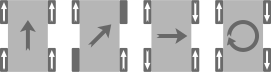
\includegraphics[width=0.8\textwidth]{graphics/mecanum_dirs.pdf}
	\caption{Podstawowe ruchy, jakie może wykonywać robot o napędzie wielokierunkowym.}
	\label{fig:mecanum_dirs}
	\end{figure} 

	Podstawa ma za zadanie transportować robota manipulującego Velma tworząc razem manipulator mobilny.
	Velma to wysoki i bardzo ciężki robot wyposażony w dwa chwytaki na ramionach o wielu przegubach, patrz fotografia \ref{fig:velma}.
	Taka budowa wymaga szerokiej podstawy, aby zachować dużą równowagę.
	Jeżdżąc na tej podstawie robot może się przemieszczać i obracać w dowolnym kierunku, aby uzyskać lepszy dostęp do manipulowanych przedmiotów.
	Dodatkowe czujniki laserowe umieszczone tuż nad postawą odpowiadają za wykrywanie kolizji i lokalizację.

	\begin{figure}[H]
	\centering
	\includegraphics[width=0.5\textwidth]{graphics/velma.png}
	\caption{Robot manipulacyjny Velma.}
	\label{fig:velma}
	\end{figure} 

	Platforma jest niesymetrycznie podzielona na dwie niezależne części, przednią i tylną w sposób pokazany na rysunku \ref{fig:base_top}.
	Przegub o jednym stopniu swobody (tzw. zawias) jest jedynym łącznikiem pomiędzy tymi dwoma fragmentami.
	Zadaniem tego przegubu jest zmniejszanie wpływu nierówności podłoża na ruch bazy, aby każde koło dociskało do podłoża z taką samą siłą, jak po drugiej stronie osi.
	Bez tego zawiasu nierówny teren uniemożliwiałby sprawne sterowanie platformą na skutek niedeterministycznego tarcia kół tej samej osi, powodując nieplanowany skręt.
	Niedeterministyczne tarcie kół jest niewykrywalne w bezpośredni sposób, więc należy je wyeliminować na przykład za pomocą takiego przegubu.

	Środki kół nie są rozmieszczone na wierzchołkach kwadratu. Jest 4 cm różnicy między szerokością, a długością.
	Szerokość jest większa, co można zobaczyć porównując widok z prawej strony \ref{fig:base_side} z widokiem z tyłu \ref{fig:base_front}.
	Dokładne wymiary są podane na rysunku \ref{fig:base_dims} i tabeli \ref{tab:dims}.

	Platforma podatna jest na losowy ruch przy rozpoczynaniu jazdy i hamowaniu.
	Jest to spowodowane tym, że asymetria rolek będzie nadawać kołom różne siły, a w związku z tym różne prędkości, co w efekcie może powodować niedeterministyczny ruch.
	Należy także wziąć tutaj pod uwagę nieprzewidywalne opory, jak nierówne tarcie rolek o powierzchnię \cite{braking}.

	\begin{figure}[H]
	\centering
	\includegraphics[width=0.5\textwidth]{graphics/base_top.png}
	\caption{Platforma mobilna --- widok od góry. Przegub zawiasowy łączy dwie części.}
	\label{fig:base_top}
	\end{figure} 

	\begin{figure}[H]
	\centering
	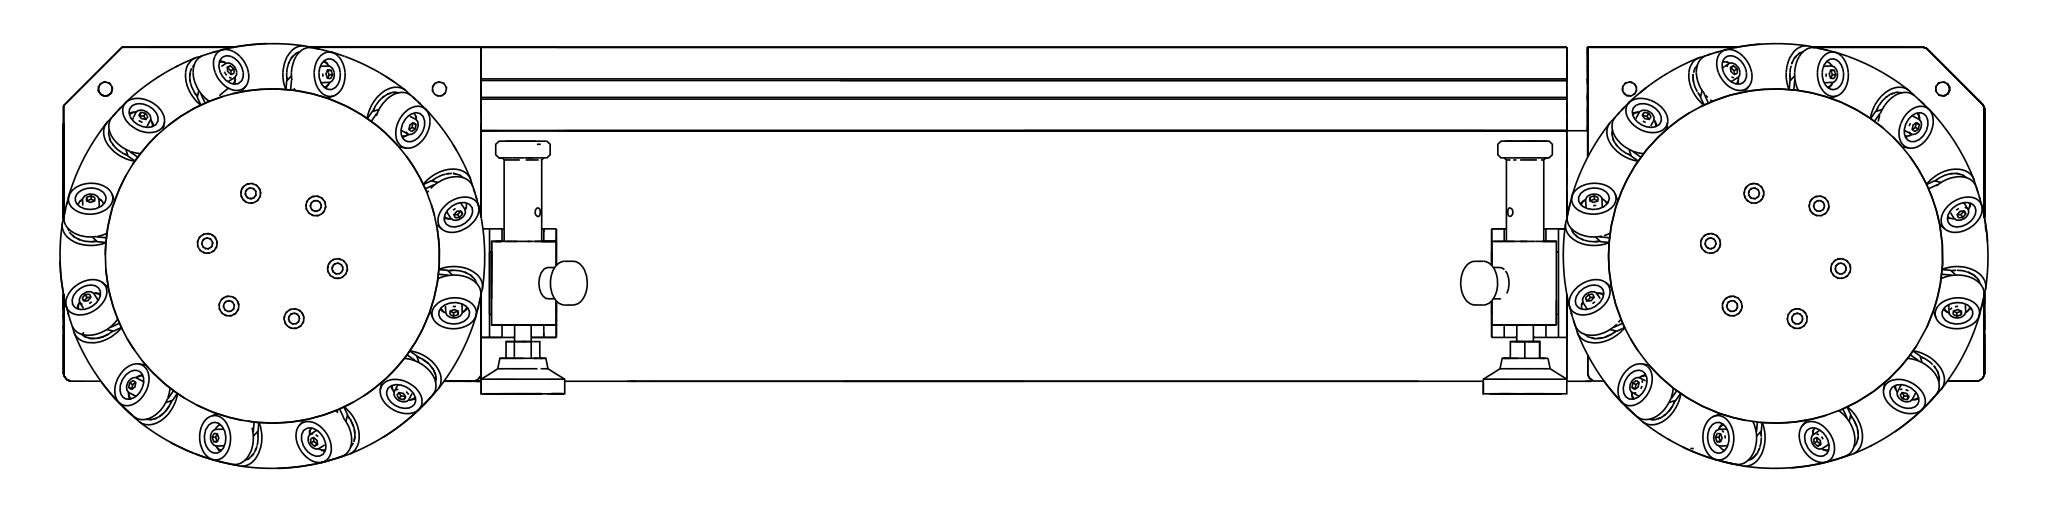
\includegraphics[width=0.5\textwidth]{graphics/base_side.pdf}
	\caption{Platforma mobilna --- widok z prawej strony.}
	\label{fig:base_side}
	\end{figure} 

	\begin{figure}[H]
	\centering
	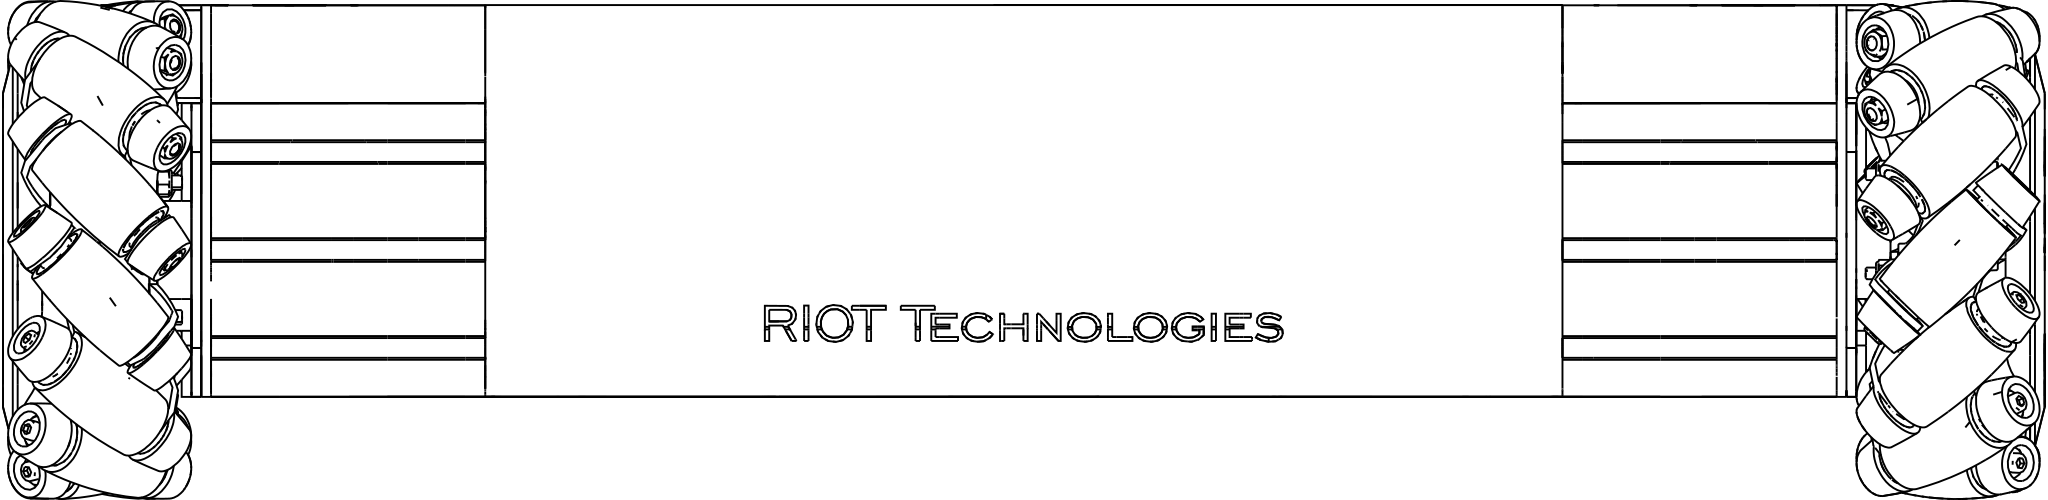
\includegraphics[width=0.5\textwidth]{graphics/base_front.pdf}
	\caption{Platforma mobilna --- widok z tyłu.}
	\label{fig:base_front}
	\end{figure} 

	Platforma posiada 3 stopnie swobody. Pierwszym i drugim jest ruch bez obrotu w osiach X i Y.
	Trzecim stopniem jest dowolny obrót po płaszczyźnie podłoża.

\section{Koła szwedzkie}
	Koła szwedzkie, zwane także kołami Mecanum, to specjalne koła z dodatkowymi rolkami na obwodzie ustawionymi pod kątem $45^\circ$ do osi koła.
	Rolki są pasywne i obracają się niezależnie od siebie. Każde koło ma 12 takich rolek, patrz rysunek \ref{fig:wheel}.
	Ich osie ustawione są w ten sposób, że osie rolek dwóch kół z tej samej strony robota przecinają się pod kątem prostym.
	Innymi słowy, robot ma identycznie ustawione koła na przeciwległych wierzchołkach, i razem ustawione są w kształt litery \emph{X} patrząc na nie z góry.
	Warto pamiętać, że oś aktualnie dolnej rolki jest prostopadła do osi górnej rolki.

	Istnieje również odwrotna odmiana ustawienia kół, w której rolki tworzą literę \emph{O}, 
	czyli oś przednia jest zamieniona z tylną, lub jakby cała platforma była odwrócona do góry nogami.
	Ten drugi sposób także pozwala na ruch wielokierunkowy, ale nie jest tak często stosowany \cite{paletobot}.

	\begin{figure}[H]
	\centering
	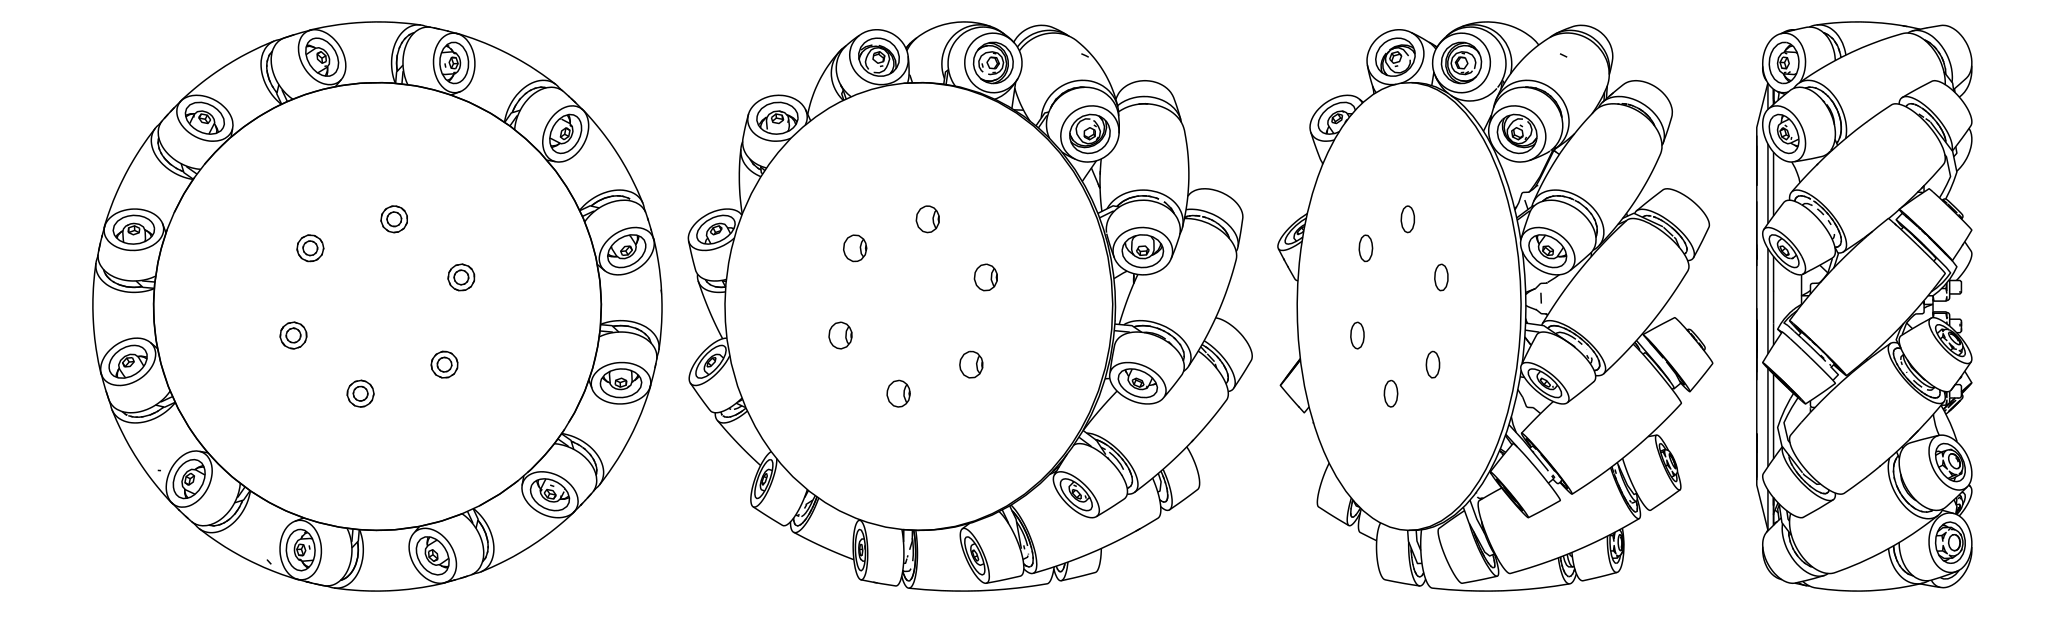
\includegraphics[width=\textwidth]{graphics/wheel.pdf}
	\caption{Widok 12 rolkowego koła szwedzkiego opisywanej platformy wielokierunkowej.}
	\label{fig:wheel}
	\end{figure} 

	Każde koło ma 3 stopnie swobody. Pierwszym jest obrót całego koła wzdłuż osi.
	Drugim są rotacje pojedynczych rolek, a trzecim poślizg obrotowy w miejscu styku rolki z podłożem \cite{kinematic_modeling}.

	Na podstawie rysunku \ref{fig:wheel} widać, że krzywizna rolki jest tak ustawiona, aby punkt kontaktu rolki z podłożem płynnie przechodził na następną rolkę w trakcie obrotu.
	Celem jest utrzymanie równej odległości osi od płaszczyzny podłoża.
	Nie powinno być efektu przeskoku z jednej rolki na drugą, gdyż to wprowadza nierówne tarcie, losowe poślizgi i nadmierne zużycie elementów wykonawczych.
	Pojedyncza rolka zawiera się w paraboloidzie, wzory opisujące kształt rolki są złożone.
	Zazwyczaj przybliża się ją torusem w celu uproszczenia produkcji \cite{rollers}.

	Istnieją także inne budowy kół, złożone z wielu małych rolek tak, aby w każdym momencie kilka rolek dotykało podłoża.
	Można także złożyć kilka powyższych kół obok siebie w jednym kole.
	Przydatne jest to dla robotów transportujących duże masy, gdyż zmniejsza to obciążenie pojedynczych rolek.
	Niestety taka budowa jest chroniona aktywnym patentem, więc pojedyncze koło, na które patent już wygasł, z jest jedynym popularnie używanym \cite{paletobot}.

	Podstawowym problemem technologicznym koła jest skomplikowana budowa, ale także ślizganie się rolek po powierzchni.
	Odległość osi od płaszczyzny nieznacznie zmienia się przy przenoszeniu ciężaru z rolki na rolkę, co przy dużych prędkościach powoduje drgania i jeszcze większe błędy pomiarów.
	Środkowy przegub zmniejsza ich przenoszenie na drugą część platformy.
	Poślizg kół powoduje, że enkodery nie mogą być jedynymi czujnikami służącymi do wyznaczania pozycji bazy, gdyż są zbyt mało dokładne \cite{heavy}.

	\subsection{Działanie}
	Standardowe koło, używając tarcia, przekształca prędkość kątową na liniową w płaszczyźnie obrotu. 
	Specjalne koło Mecanum ma dodatkowy wektor równoległy do osi obrotu, zatem prędkość wypadkowa jest obrócona o 45°, zależnie od typu koła (prawoskrętne lub lewoskrętne) i 
	kierunku obrotu.

	\begin{figure}[H]
	\centering
	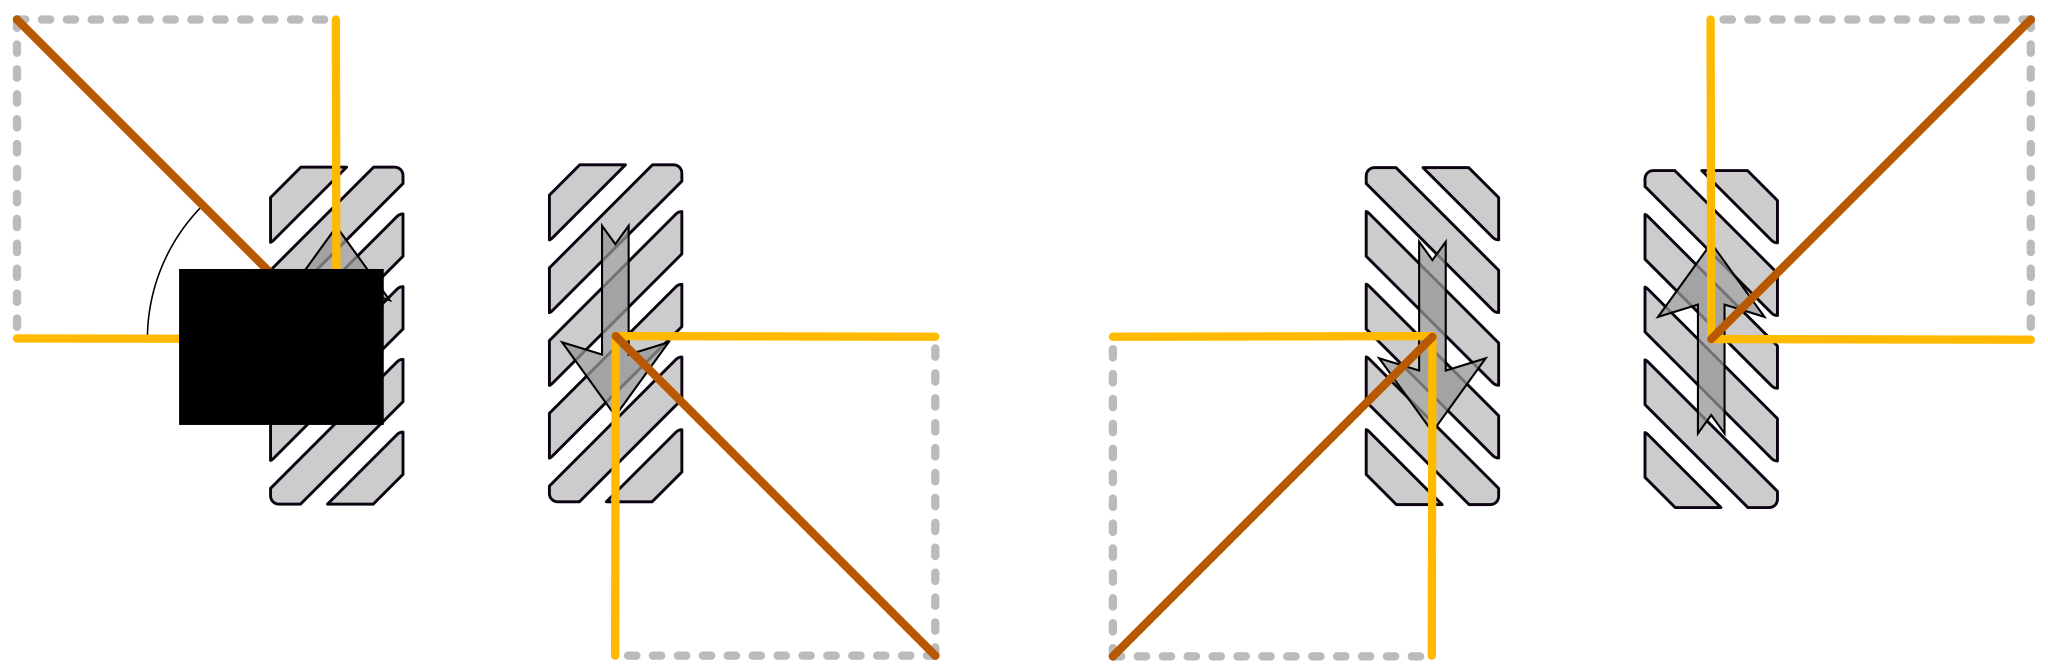
\includegraphics[width=\textwidth]{graphics/vectors.pdf}
	\caption{Wektory składowe i wypadkowe koła widzianego z góry.}
	\label{fig:wheel_vectors}
	\end{figure} 

	Ustawiając te koła w odpowiedni, opisany wcześniej na obrazku \ref{fig:base_top}, sposób można zmusić wektory kół do odpowiedniego znoszenia się składowych,
	a w efekcie pozwolić robotowi na poruszanie się w kierunkach nieosiągalnych dla pojazdów o standardowych kołach.
	A zatem, można nałożyć te składowe na wcześniejszy rysunek \ref{fig:mecanum_dirs} i dokładnie się przyjrzeć, dlaczego koła popychają przy danym obrocie platformę w 
	danym kierunku.

	\begin{figure}[H]
	\centering
	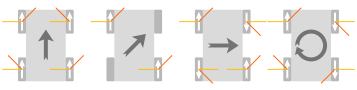
\includegraphics[width=\textwidth]{graphics/mecanum_dirs_vect.pdf}
	\caption{Wektory składowe i wypadkowe piasty koła widzianego z góry.}
	\label{fig:mecanum_dirs_vect}
	\end{figure} 

	W pierwszym przypadku, wektory o kierunku prostopadłym do płaszczyzny symetrii urządzenia znoszą się, pomimo że mają przeciwne zwroty na przedniej i tylnej parze kół.
	Pozostają jedynie składowe równoległe do płaszczyzny symetrii, które powodują prostoliniowy ruch w przód.

	Drugi przypadek jest podobny, lecz dwa koła nie obracają się. Nie jest to ruch pasywny, gdyż taki wprowadzałby nieprzewidywane poślizgi, a aktywne hamowanie.
	Wtedy wektory nie mają się jak znosić i platforma wykonuje ruch pod kątem 45° do płaszczyzny symetrii.

	Zasada ruchu w bok jest bardzo podobna do ruchu w przód. Tutaj również wektory znoszą się parami, jednak tym razem na prawych kołach i lewych.

	Alternatywnie, bardzo łatwo nadać prędkość kątową podstawie przy odpowiednim ustawieniu prędkości kół.

	Warto nadmienić, że w idealnym przypadku rolki nie obracają się, gdy wypadkowy wektor prędkości koła jest prostopadły do osi koła. 
	Inaczej mówiąc, rolka będzie się obracać tym mocniej, im bardziej ruch koła wymuszany jest równolegle do osi koła, 
	czy to na skutek znoszenia się wektorów, czy oporu przeszkody.
	I na przykład, przy ruchu w przód rolki koła praktycznie się nie obracają, lecz przy ruchu w bok biorą aktywny udział.
	Może mieć to wpływ na zużywanie się rolek, nie tylko z punktu widzenia ilości obrotów danej rolki na pokonanym dystansie, 
	ale także sposobu w jaki wymuszany jest jej ruch.
	Rolki zawsze będą nieznacznie się obracać nieco szarpanym ruchem w obie strony, ze względu na poślizgi od innych kół, 
	niejednostajne tarcie piast wszystkich innych rolek, czy różnice terenu. 
	Zatem przejazd przykładowego odcinka przodem lub bokiem, będzie w różnym stopniu i w różny sposób zużywał elementy wykonawcze.
	To, jaki styl jazdy opłaca się zastosować, aby zminimalizować zużywanie się elementów jest dużą, odrębną dziedziną nauki.

\section{Czujnik laserowy}
	\label{sec:lidar}
	Program sterujący platformą nie jest w stanie dokładnie określić pozycji robota, bazując jedynie na odometrii.
	Potrzebny jest zatem czujnik laserowy.
	Platforma wyposażona jest w dwa, dwuwymiarowe czujniki typu LiDAR firmy SICK.
	LiDAR to zbitek wyrazów \emph{light} i \emph{radar}, chociaż skrót może być rozwinięty w różne słowa.

	\begin{figure}[H]
	\centering
	\includegraphics[width=0.5\textwidth]{graphics/sensor.png}
	\caption{Czujnik laserowy SICK LMS100-10000.}
	\label{fig:sensor}
	\end{figure} 

	\subsection{Zasada działania}
	Wszystkie czujniki tego typu mają bardzo podobną zasadę działania.
	Pośrodku urządzenia znajduje się obrotowe lusterko, zwrócone pod kątem 45° do osi obrotu.
	Równolegle do osi znajduje się laser, który emituje pulsacyjną wiązkę podczerwonego promienia co pewien okres.
	Aktualna pozycja lusterka jest wykrywana przez enkoder.
	Obok lasera jest czujnik, który bada wysłane przez laser, odbite od lusterka, obiektu i ponownie lusterka, światło.

	Na koniec zaawansowany algorytm we wbudowanym mikrokontrolerze ustala kąt i odległość wykrytego obiektu.
	Odpowiada także za usunięcie szumu i ewentualnych odbić promienia.
	Komunikacja odbywa się za pomocą różnych interfejsów sieciowych, zazwyczaj w architekturze master-slave.

	\subsection{Komunikacja}
	Wysyłając do czujnika odpowiedni ciąg bajtów, można ustawić jego tryb działania, odpytać o zebrane dane, czy wykryć konfigurację i stan.

	W przypadku naszej platformy, komunikacja odbywa się poprzez interfejs Ethernetowy.
	Program komunikujący się bezpośrednio z urządzeniem zwraca pakiety zawierające pomiary z ostatniego obrotu czujnika, oraz dane 
	opisujące sam pomiar takie jak czas, początkowy kąt pomiaru, tryb itp.
	Dokładne dane i cechy czujnika dostępne są na stronie producenta \cite{sick_website}.

	Urządzenie wspiera uwierzytelnianie przez hasło, wgrywanie nowego oprogramowania,
	ustawienia czasu, oraz zmianę różnych parametrów działania.

	\subsection{Podstawowe cechy}
	Czujnik składa się z dwóch części, głównego trzonu oraz nakładki.
	To powoduje, że nie może mierzyć w kącie pełnym i powstaje martwa strefa.
	Przedstawia to dobrze grafika producenta.
	\begin{figure}[H]
	\centering
	\includegraphics[width=0.6\textwidth]{graphics/sick.png}
	\caption{Wykres producenta dotyczący zasięgu czujnika.}
	\label{fig:lidar}
	\end{figure} 
	
	\begin{table}
	\centering
	\begin{tabular}{l r}
	Cecha & Wartość \\
	\hline
	Kąt pracy & 270\textdegree \\
	Długość fali światła lasera & 905 nm (podczerwień) \\
	Częstotliwości skanowania & 25 Hz / 50 Hz \\
	Maksymalna odległość obiektu & $\approx$ 20 m \\
	Rozdzielczość kątowa & $0,25 \degree$ / $0,5 \degree $ \\
	Systematyczny błąd pomiarowy & $\pm 0,03$ m \\
	Przypadkowy błąd odległości & $0,012$ m \\
	\end{tabular}
	\caption{Podstawowe cechy czujnika laserowego.}
	\label{tab:lidar}
	\end{table}
	Urządzenie jest w stanie komunikować się za pomocą portu szeregowego RS-232, połączenia Ethernetowego i sieci CAN.

\section{Składniki systemu}
	Środowisko symulacyjne składa się z kilku odrębnych modułów, które komunikują się ze sobą poprzez specjalne interfejsy wykorzystujące kolejki wiadomości.
	Taka implementacja komunikacji pozwala zmieniać i reimplementować poszczególne elementy i używać różnych języków programowania zachowując tę samą komunikację między składnikami nie tracąc kompatybilności między sobą.
	Możliwe jest także przesyłanie wiadomości przez sieć, co pozwala na rozproszenie systemu.

	%TODO Zmienić na Tikz
	\begin{figure}[H]
	\centering
	\includegraphics[width=0.8\textwidth]{graphics/agent.pdf}
	\caption{Struktura agenta upostaciowionego.}
	\label{fig:agent}
	\end{figure} 

	Można to przedstawić za pomocą zapisu agentowego, jak na rysunku \ref{fig:agent}.
	Agent upostaciowiony składa się wilku modułów komunikujących się ze sobą za pomocą różnych systemów.

	Nadrzędnym modułem jest układ sterowania, który na podstawie odczytów z czujników generuje sterowanie dla efektorów.
	Ważne jest, aby komunikacja z rzeczywistymi urządzeniami była identyczna, jak z ich modelami, dzięki czemu taki system będzie przenośny i niezależny.

	Efektor rzeczywisty, na przykład serwomotor, jest sterowany za pomocą efektora wirtualnego, który zamienia wyjście układu sterowania na sygnały sterujące dla silnika napędowego.
	Przykładowo zmienia podaną liczbę oznaczającą zadaną prędkość na odpowiednie napięcie na wyjściu.

	Zamodelowany efektor symulowany również przyjmuje te same sygnały do układu sterowania, lecz nie zamienia ich na sygnały sterujące, a wywołuje odpowiednie funkcje maszyny symulacyjnej nadające siły i prędkości obiektom w przestrzeni wirtualnej.

	Receptor wirtualny pobiera surowe dane z czujnika, przekształca na odpowiedni format, usuwa błędy i szum tak, aby program sterujący mógł wykorzystać te dane w prosty sposób. 
	Doskonałym przykładem jest tutaj kamera Kinect, w której to zachodzi odczytanie obrazu z kilku kamer.
	Następnie obraz przesyłany jest do komputera w którym sterowniki interpretują dane usuwając błędy, tworzą mapę głębokości, wykrywają szkielety i sylwetki osób.
	Te dane mogą być wykorzystane łatwo w grach i programach sterujących.

	Modelowanie receptora, tak jak w przypadku efektora polega na wygenerowaniu odpowiednich danych używając odpowiednich funkcji w przestrzeni wirtualnej.
	Mogą one polegać na puszczaniu promieni symulujących laser, lub wręcz renderowaniu obiektów, aby uzyskać obraz z wirtualnej kamery.
	Receptor symulowany ma pełną wiedzę o symulowanym świecie, dokładne pozycje i prędkości wszystkich obiektów, dane o kolizjach itp. 
	Pozwala to na łatwe symulowanie receptorów nie mogących mieć odwzorowania w rzeczywistości, co przydatne jest w pierwszych stadiach testowania i wyznaczaniu statystyk.

	\subsection{Model 3D}
	Model 3D bazy mobilnej opisany równaniami matematycznymi powinien mieć zachowanie najbardziej jak to tylko możliwe zbliżone do oryginału.
	Musi uwzględniać masy i momenty bezwładności elementów składowych, a także wszystkie tarcia.
	Model obejmuje więzy na ruchome elementy, takie jak koła i rolki, aby umożliwić symulację przegubów.

	Model składa się z elementów odwzorowujących rzeczywiste części składowe bazy mobilnej.
	Elementy posiadają takie cechy, jak pozycja w modelu, masa, moment bezwładności, kształt, materiał fizyczny i wygląd.
	Dodatkowo należy uwzględnić więzy tych składowych w postaci symulowanych przegubów.
	W przypadku tej bazy istnieje jeden typ więzów o jednym stopniu swobody (zawias).
	Więzy mogą oddziaływać siłą na elementy do których są podłączone symulując silniki.

	Elementy składowe i symulowane przeguby oddziałują bezpośrednio z maszyną do symulacji fizycznej. 
	To kształt, masy i momenty bezwładności brył są argumentami funkcji liczących.
	Maszyna symulacyjna oblicza odpowiednie prędkości i nadaje podanym obiektom w podobny sposób, jak ma to miejsce w rzeczywistości.

	Do modelu doczepia się wirtualne czujniki generujące odpowiednie dane na podstawie symulacji i rozkładu losowego.
	Nie są to pełne dane o stanie modelu, jakie posiada maszyna do symulacji, gdyż czujniki fizyczne również nigdy nie mają pełnej informacji o stanie urządzenia.
	Należy dodać losowy szum i błędy, aby przybliżyć ich zachowanie do rzeczywistych czujników.

	Dla ozdoby można wykorzystać istniejący model CAD do stworzenia siatki trójwymiarowej i nadania symulowanemu obiektowi wyglądu zbliżonego do fizycznego robota.

	\subsection{Sterownik silników}
	Program sterujący generuje abstrakcyjne dane, na przykład liczbę zapisaną binarnie.
	Przykładowy silnik fizyczny nie jest w stanie działać na ich podstawie, on potrzebuje odpowiedniego napięcia na wejściu.
	Do tłumaczenia jednych danych na drugie potrzebny jest sterownik niskopoziomowy.
	Najczęściej implementowany jest w formie mikrokontrolera, lub podobnego systemu wbudowanego.

	Jego zadanie to odczytanie danych podanych przez program sterujący i na przykład generowanie na ich podstawie odpowiedniej fali PWC, lub obsługa przetwornika cyfrowo-analogowego.
	Do innych zadań może należeć kontrola, czy żądana wartość nie uszkodzi urządzenia.
	Zazwyczaj sterownik może komunikować się z powrotem z resztą systemu, aby zgłaszać ewentualne awarie.

	Taki program i powiązany z nim układ elektroniczny są najczęściej dostarczone przez producenta robota i nieznane użytkownikowi.
	Dodatkowo tworzy kolejną warstwę abstrakcyjną dla sterownika głównego, który nie musi zważać na generowanie różnych danych dla różnych modeli tych samych efektorów.
	
	W środowisku wirtualnym należy stworzyć moduł o podobnym działaniu.
	Powinien przyjmować dane w dokładnie takim samym formacie, jak opisany wyżej układ, aby był łatwo wymienialny na sterownik fizycznego urządzenia bez ingerencji w główny program sterujący.
	Zamiast zamieniać odczytane dane na analogowe wartości, on wywołuje odpowiednie funkcje maszyny symulacyjnej, aby wywołać taki sam efekt, co na rzeczywistym efektorze, lecz w wirtualnej przestrzeni symulacji.
	Jako argumenty podaje parametry fizyczne symulowanego obiektu, oraz przyłożone siły.
	

	\subsection{Sterownik czujników}
	Implementowany podobnie do sterownika silników ma za zadanie konwertować surowe i obarczone błędami dane z czujników na format zrozumiały dla programu sterującego.
	W tym miejscu usuwa się błędy grube, niweluje stałe na podstawie kalibracji, wygładza szum i interpretuje dane, aby pozyskać wymagane przez wyższe warstwy informacje.

	Przykładowo czujniki laserowe zwracają jedynie ciąg pomiarów, ale to do tego programu należy interpretacja wykrytych kształtów, łączenie punktów i obróbka do formatu zrozumiałego dla wyższych podzespołów.
	Większość zaawansowanych receptorów posiada owe układy cyfrowe i programy wbudowane w urządzenie.
	Dostarczone przez producenta tak samo, jak sterowniki efektorów.
	
	Symulując ten element budujemy program generujący dane na podstawie aktualnego stanu maszyny do symulacji w sposób, w jaki działa czujnik w rzeczywistości.
	Na przykład dla czujnika laserowego wypuszczamy setki promieni i obliczamy ich punkty przecięcia się z wirtualnymi modelami.
	Możemy renderować obraz, aby symulować kamerę.

	Ponieważ dane fizyczne nigdy nie są idealne, w celu przybliżenia wyjścia wirtualnego czujnika do oryginału, dodajemy szum o odpowiednim rozkładzie i błędy.

	\subsection{Program sterujący}
	Cześć odpowiedzialna za logikę aplikacji. Tutaj obliczane jest sterowanie na podstawie dostarczonych odczytów z czujników.
	Zazwyczaj wykorzystuje się tu dużą ilość bibliotek dostarczających zaawansowane algorytmy.
	Ich zadania mogą polegać na budowie wewnętrznej mapy, wyznaczaniu ścieżki, omijaniu przeszkód, odwrotnej kinematyce i tym podobnych.

	Taki program zwykle działa na mocniejszych układach, niż sterowniki ze względu na duże zapotrzebowania na moc obliczeniową.
	Jeśli robot komunikuje się z użytkownikiem, lub zwraca dane, to zachodzi to w tym module. 

	Programy sterujące mogą być implementowane w językach wysokopoziomowych, nawet skryptowych, gdyż wymagania czasowe nie są rygorystyczne.
	Co więcej, często się zdarza, że odpowiednie składowe programu bazują na różnych technologiach.

	Środowisko symulacyjne powinno zapewnić pełną abstrakcję komunikacji tego modułu.
	Oznacza to, że niezależnie, czy program działa na rzeczywistym robocie, czy symulacji wirtualnej, zawsze powinien móc komunikować się i otrzymywać dane w tym samym formacie.
	W idealnym świecie program nie powinien mieć możliwości stwierdzić, czy steruje symulacją, czy oryginałem.

\section{Technologie}
	Symulator daje użytkownikowi do dyspozycji odpowiednią maszynę symulacyjną odpowiedzialna za obliczenia fizyczne, a także API do obsługi całej symulacji.
	Zaawansowana maszyna symulacyjna powinna dobrze obsługiwać tarcia, więzy na ruch obiektów, przyłożone siły, materiały fizyczne dla określania tarcia i sprężystości, 
	oraz wszystko to, co potrzebne do jak najwierniejszego odtworzenia zachowania rzeczywistego obiektu.

	Na rynku jest wiele różnych maszyn zarówno do symulacji w czasie rzeczywistym, jak i do wyznaczania pozycji obiektów po długich obliczeniach.
	Jedne z technologii są otwartoźródłowe, inne nie. Mogą używać tylko procesora, lub też być wspomagane przez kartę graficzną.
	Niektóre prócz zderzeń obiektów potrafią także symulować rozpływ cieczy, dymy, płótna, ciała sprężyste i strukturę wewnętrzną obiektów, lecz te funkcjonalności nie są potrzebne dla naszej symulacji.

	\subsection{Gazebo}
	Program do pobrania z \cite{gazebo_website}. Ten symulator graficzny jest dość prosty w obsłudze, skupia się na symulowaniu podanych danych, a mniej na możliwości ich łatwego przygotowania.
	Zazwyczaj używany w trybie wsadowym, uruchamiany z argumentami z linii poleceń i plikiem \emph{world} opisującym symulację.
	Plik ten zawiera nazwy i ścieżki innych umieszczanych modeli i wtyczek.
	Z tego powodu interfejs graficzny jest dość ubogi.

	Program przeprowadza symulację podanych modeli używając jednego z czterech popularnych maszyn symulacyjnych: ODE, Bullet, Simbody lub DART.
	Wszystkie te projekty są wolnym oprogramowaniem i używane są także w innych programach, jak Blender.

	Symulator oprócz tego ma wbudowany edytor modeli w którym możemy składać odpowiednie obiekty od razu w przestrzeni trójwymiarowej.
	Edytor budynków pozwala na stawianie wirtualnych ścian, korytarzy, drzwi i ogólnego otoczenia w którym roboty mogą pracować i być symulowane.
	Jakość wykonania tych składników pozostawia wiele do życzenia, brak jest tak podstawowych funkcji, jak cofanie ruchu.
	Dlatego lepiej jest definiować model we wczytywanym pliku tekstowym.
	Również tworząc modele poza edytorem w ten sposób mamy nad nimi pełną kontrolę, a parametry można ustawiać z dowolną dokładnością.

	Gazebo przyjmuje modele w specjalnym formacie SDF. Jest to ustandaryzowany, zdefiniowany zewnętrznie format do opisywania składników robotów i czujników.
	Dzięki temu taki plik może być użyty także gdzie indziej, pod warunkiem przestrzegania standardu.
	Składnia jest zwykłym plikiem XML, co znaczy, że może być on tworzony na każdym edytorze tekstowym.

	Wtyczka do sterowania modelem jest skompilowaną biblioteką dołączaną na starcie programu.
	Tworzy się ją w C++ jako klasę dziedziczącą po abstrakcyjnej klasie dostarczonej przez Gazebo.
	Dzięki temu może się komunikować z innymi systemami poprzez dowolne mechanizmy, nawet systemowe, jak gniazda, czy pamięć współdzielona.
	Jednak Gazebo dostarcza także swój własny mechanizm kolejek wiadomości, który sprawdza się w jednolitej komunikacji z innymi programami.

	Program jest wspierany na systemie Ubuntu ale bez problemu można go także skompilować pod inne systemy.
	Interfejs jest dopracowany i przestrzega wielu ustawień systemowych, jak DPI.
	Uruchamianie jest proste i nie wymaga dodatkowych ustawień, uruchamiania skryptów inicjalizujących, tworzenia odpowiednich katalogów, czy definiowania zmiennych systemowych.
	Standardowo, jak inne programy tworzy ukryty katalog w katalogu domowym użytkownika, gdzie znajdują się wszystkie modele i logi.
	Czasami trzeba używać tego katalogu, aby umieścić tam swoje modele, które Gazebo będzie automatycznie umieszczał w symulacji.

	Gazebo jest składnikiem systemu ROS, kod źródłowy jest dzielony w ramach wspólnej organizacji, chociaż różne osoby odpowiadają za rozwój tych oprogramowań.
	Kolejne wersje Gazebo są powiązane z wersjami ROSa, nie można użyć przestarzałej wersji Gazebo z nowszym ROSem i odwrotnie.
	Symulator można zainstalować osobno, lub jako jeden z pakietów ROSa.

	\subsection{V-Rep}
	Program do pobrania z \cite{vrep_website}. Duże i skomplikowane środowisko reklamujące się wieloma zaawansowanymi mechanizmami i funkcjami.
	Pomimo otwartego kodu, użycie komercyjne jest płatne. Dla zastosowań akademickich program jest rozdawany bez opłat.
	Bogaty interfejs graficzny zakłada budowę i symulację wszystkiego w tym jednym programie.

	Używa dwóch z maszyn symulacyjnych, co Gazebo, czyli ODE i Bullet, oraz dodatkowo Vortex i Newton. Z tej czwórki tylko Vortex ma zamknięty kod.

	Problemem jest także zapisywanie utworzonych w systemie modeli.
	Program tworzy drzewiastą strukturę modelu w pliku binarnym własnego formatu, co uniemożliwia edycję i oglądanie modelu bez posiadania całego programu i importowania modelu do symulacji.
	Brak przenośności, czy wsparcia systemu kontroli wersji dla takich zbiorów bajtów także jest problemem.

	Pisanie wtyczek najczęściej odbywa się w C. Są też jednak dostępne inne języki skryptowe, jak Lua, Matlab, Java itp.
	Komunikacja z innymi programami odbywa się poprzez specjalne dodatki do środowiska.
	API pozwala nam stworzyć mały, wbudowany interfejs graficzny do sterowania symulacją poprzez przyciski i suwaki.

	Ze strony producenta pobieramy gotowe archiwum z programem, który nie wymaga żadnej instalacji i posiada wszystkie potrzebne zasoby do pracy i nauki, jak przykładowe modele istniejących komercyjnych robotów.
	Program działa w trzech najpopularniejszych systemach operacyjnych --- Windows, Linux i OS X.

	\subsection{ROS}
	Platforma programistyczna do pobrania z \cite{ros_website}.
	ROS jest skrótem od \emph{Robot Operating System}, lecz jego nazwa jest bardzo myląca.
	Nie jest to żaden system operacyjny, lecz obszerna platforma programistyczna (framework) zawierająca odpowiednie biblioteki i narzędzia do tworzenia programów sterujących.
	ROS stara się w łatwy sposób dostarczyć wszystko, co potrzebne do budowy logiki aplikacji sterowania.
	Są tu algorytmy wyznaczania tras, budowy map, manipulowania itp. 

	Twórcy zachęcają, aby uzupełniać brakujące moduły swoimi własnymi, a potem dzielić się nimi z resztą programistów, aby każdy mógł skorzystać, jeśli ma podobny problem.

	Programy dla ROS pisze się w C++, lub Pythonie i integruje z robotem za pomocą kilku gotowych struktur kolejek wiadomości.
	Platforma ta także posiada moduły do wizualizacji odbieranych danych w formie graficznej.
	Nie jest to symulator, gdyż sam nie generuje żadnych danych, a jedynie prezentuje gotowe.

	Działanie systemu jest oparte o pakiety. Każdy pakiet jest katalogiem zawierającym w sobie pliki opisujące jego parametry i skrypty używane w kompilacji.
	Pakietem może być wszystko, od modelu do programu pomocniczego.
	Pakiety mogą być zależne od siebie, ale nigdy nie wskazują nawzajem swoich bezpośrednich ścieżek.

	Na przykład, jeden pakiet wymaga pliku nagłówkowego generowanego przez kompilację drugiego pakietu, ale załącza go w kodzie tak, jakby był systemowy.
	Globalny skrypt kompilacji ROSa dba o odpowiednie podawanie ścieżek, kolejność kompilacji programów i załączanie nazw.

	Komunikacja między programami odbywa się w sposób ciągły przez kolejki wiadomości, lub pojedyncze asynchroniczne wywołania zwracające wynik.
	Program może nadawać strumień wiadomości, ale niekoniecznie musi istnieć w tym czasie odbiornik.
	Można buforować wiadomości, podglądać strumienie, tworzyć wykresy z danych, podłączać nadajnik do kilku odbiorników, podglądać graf zależności itp.
	Do wszystkiego służy bogaty zestaw komend.

	Instalacja programu na systemie operacyjnym jest dużym problemem.
	Z wyjątkiem odpowiednich wersji Ubuntu nie ma łatwego sposobu na wgranie go do innych systemów.
	Na przeszkodzie stoją błędy kompilacji dla nowszych wersji kompilatorów i inne problemy w czasie wykonywania, jak naruszenie ochrony pamięci. 
	Instalacja alternatywnych pakietów i ręczna kompilacja niektórych części nie działa we wszystkich przypadkach.
	Głównym problemem jest niezgodność wersji zewnętrznych bibliotek.

	Rozwiązaniem tego problemu jest instalacja tej platformy programistycznej na maszynie wirtualnej, lub na systemie uruchamianym z dysku zewnętrznego. 
	Takie rozwiązanie także daje dostęp do najnowszej wersji długiego wsparcia ROS \emph{Kinetic Kame} z końca maja 2016 roku.

	Uruchomienie platformy programistycznej na systemie wymaga wielu dodatkowych komend inicjalizujących, a także dopisywania do tworzonych projektów licznych plików konfiguracyjnych za pomocą dostarczonych skryptów.
	Używanie modułów z linii poleceń wymaga ustawienia kilku zmiennych systemowych poprzez wczytywania całościowych plików.
	Użycie niektórych funkcji ROS wymaga uruchomionego demona serwera w tle.

	Ogólnie instalacja i używanie ROS na systemie zostawia dużo różnorodnych plików w katalogu domowym, dlatego lepiej jest trzymać ją z dala od codziennego systemu operacyjnego, na maszynie wirtualnej, lub dysku.
	Z drugiej jednak strony wirtualizacja systemu operacyjnego z ROS bardzo ogranicza dostępną moc obliczeniową potrzebną takim programom w dużych ilościach.

	\subsection{Narzędzia}
	Do tworzenia oprogramowania na systemach Unixowych można użyć dowolnych edytorów, gdyż standardowo wszystko jest potem kompilowane za pomocą narzędzi wiersza poleceń i skryptów.
	Jednak warto sobie ułatwić pracę zaawansowanymi środowiskami graficznymi.
	\begin{description}
	\item[Gazebo] będzie użyty do symulacji z jego domyślną maszyną symulacji fizyki ODE.
	\item[ROS] użyty zostanie jako gówna platforma programistyczna. Pod łatwą komunikację z jego modułami należy budować sterowniki wirtualne.
	\item[Atom] jest popularnym uniwersalnym edytorem tekstowym. Dzięki rozszerzaniu przez wtyczki dobrze się sprawdza przy obróbce plików XML i skryptów.
	Będzie użyty do konstrukcji modelu.
	\item[CMake] to popularny i polecany przez ROS i Gazebo system budowy kodu. Program tworzy na podstawie swoich plików konfiguracyjnych plik \texttt{makefile} do kompilacji źródeł i łączenia bibliotek.
	\item[GCC] będzie użyty do kompilacji, gdyż jest to najpopularniejszy tego typu program używany w GNU/Linux. Same symulatory zostały w nim skompilowane.
	Razem z nim użyty zostanie debugger GDB. 
	\item[KDevelop] nadają się do pisania kompilowalnego kodu wtyczek. Można podłączyć je pod komendę \texttt{make} i korzystać z mechanizmów interpretacji błędnych wierszy, graficznego debugowania i podobnych.
	\item[Bash] będący bardzo popularnym językiem skryptowym nadaje się do automatyzacji pracy i uruchamiania wielu programów w kontrolowany i szybki sposób.
	Uniwersalne narzędzie pomagające w różnych miejscach.
	\item[Git] jest narzędziem kontroli wersji, które jest wskazane w każdym projekcie informatycznym. Kod należy dla bezpieczeństwa umieszczać także w usłudze GitHub.
	\item[Virtualbox/Qemu] do ewentualnej wirtualizacji systemu operacyjnego z ROS, lub uruchomienie osobnego systemu z dysku zewnętrznego.
	\end{description}

\section{Plan pracy}
	\begin{enumerate}
	\item Należy stworzyć model w SDF zachowując wszystkie rozmiary i momenty rzeczywistej wersji.
	Bryły składowe modelu muszą przypominać kształtem części z których składa się robot, należy im także ustawić parametry fizyczne, jak masę, moment bezwładności, materiał itp.

	\item Zamodelować wszystkie więzy na koła, rolki i przegub, aby maszyna symulacyjna poprawnie symulowała obiekt.
	Taki model powinien na tym stanie poprawnie reagować na wirtualne siły, lecz jego efektory nie będą jeszcze aktywne.
	Można go prosto pobieżnie przetestować działając siłą na elementy i patrząc, czy reagują w spodziewany sposób.

	\item Zapisanie wtyczki sterującej w Gazebo odczytującej odpowiednie dane z zewnątrz i wywołującej funkcje maszyny symulacyjnej, aby modyfikować ruch modelu.
	Na tym poziomie można dobudować zamiennik programu sterującego jedynie do podawania prostych wartości bez odczytywania pomiarów i sterowania.

	\item Zaprogramowanie wtyczki symulującej czujniki, aby generowały dane z enkoderów, oraz innych urządzeń, dodawały błędy pomiarowe, a następnie przekształcały dane na format zrozumiały dla programu sterującego.
	Czujniki nie muszą być istniejące, mogą generować dane, jak pozycja i rotacja bardzo trudne do uzyskania rzeczywistymi czujnikami.

	\item Wystawienie do zmiany w czasie rzeczywistym masy, momentu bezwładności, współczynników tarcia, aby pozwolić na proste testowanie działania systemu z różnymi współczynnikami.

	\item Elementy pomagające w symulacji, jak model kinematyczny sterowany funkcją matematyczną i podłoże ze zmiennym współczynnikiem tarcia.

	\item Programy pomocnicze zbierające i wyświetlające dane, interfejs graficzny.

	\item Program sterujący w ROS. Największy i najbardziej skomplikowany element, na szczęście wspólny dla obu bytów --- wirtualnego i rzeczywistego.
	Zazwyczaj nie jest to praca jednego człowieka, a jego rozwój nie ustaje przez długi czas.
	Ten program dostarczy funkcji, aby wyższy sterownik robota mógł użyć tego modułu do sterowania jazdą i odczytywania danych.
	\end{enumerate}

\section{Istniejące implementacje}
	Istnieją już wcześniejsze modele jeżdżących robotów na kołach szwedzkich.
	Można z nich brać przykład i sugerować się źródłami kodu i modeli.

	Kuka Youbot jest popularnym robotem wielokierunkowym. Jego modele są domyślnie dostępne zarówno w Gazebo, jak i w V-Rep.
	Tylko w przypadku V-Rep mamy wstępny sterownik do którego wysyłamy odpowiednie wartości kierunku, a on nadaje takie prędkości kołom, aby poruszać się w zadanym kierunku.
	Wersja dla Gazebo jest statycznym modelem z błędnie ustanowionymi przegubami, jego efektory nie są zaimplementowane.

	Te profesjonalne modele także pomogą przy wstępnej weryfikacji zachowania się naszego modelu, czy nie zachowuje się nadzwyczaj dziwnie w pierwszych fazach projektu.

	Ze względu na niezwykle zaawansowany obiekt kół i kształt rolek, prawdopodobnie trzeba będzie uprościć model poprzez zamianę niektórych składowych i dodanie sztucznych więzów.
	Całościowy model może być zbyt skomplikowany, aby maszyny symulacji mogły go obliczać w czasie rzeczywistym.
	Taki model także jest znacznie trudniej poprawnie wymodelować ze względu na liczne tarcia i poślizgi rolek.

\chapter{Baza}
\label{sec:robot}
\section{Dookólna platforma mobilna}
	\begin{figure}[H]
	\centering
	\includegraphics[width=0.8\textwidth]{graphics/base_photo.png}
	\caption{Dookólna baza mobilna na kołach szwedzkich.}
	\label{fig:base_photo}
	\end{figure} 

	Jest to duża, prostokątna baza dookólna, poruszająca się na czterech kołach szwedzkich, patrz fotografia \ref{fig:base_photo}.
	Koła są stałe, parami przytwierdzone do dwóch osi.
	Każde koło jest sterowane osobno przez podłączony bezpośrednio serwomotor, 
	zatem może mieć prędkość i kierunek niezależny od prędkości pozostałych kół, kierunku poruszania się robota, oraz jego obrotu.
	Każdy z serwomotorów ma także wbudowany enkoder.
	Sterownik enkodera zwraca aktualny kąt i prędkość obrotu.

	Jest to najpopularniejsza budowa dookólnych platform mobilnych, mająca zastosowanie także w innych robotach, jak na przykład Kuka Youbot \ref{fig:kuka_youbot}.
	Istnieją także roboty o trzech kołach szwedzkich, w których to koła rozstawione są promieniście pod kątami 120°.
	Pomimo prostszej budowy i takiej samej ilości stopni swobody, co czterokołowa wersja, stabilność takiego rozwiązania jest gorsza od zastosowanej tutaj budowy \cite{extra_axis}.
	Ponieważ jest to robot transportowy, to stabilność odgrywa tu ważną rolę i czterokołowa budowa jest wskazana.

	\begin{figure}[H]
	\centering
	\includegraphics[width=0.5\textwidth]{graphics/kuka_youbot.png}
	\caption{Przykład innej platformy wielokierunkowej na podstawie fragmentu komercyjnego robota Kuka Youbot. 
	Należy zwrócić uwagę na charakterystyczne ustawienie kół, identyczne jak w opisywanej platformie \ref{fig:base_photo}.}
	\label{fig:kuka_youbot}
	\end{figure} 

	Odpowiedni obrót kół względem bazy, pozwala na jej ruch w dowolnym kierunku, niezależnym od kąta obrotu robota, patrz rysunek \ref{fig:mecanum_dirs}.
	Jest możliwe także obracać bazą, gdy ta porusza się w dowolnym kierunku, bądź stoi w miejscu.
	
	\begin{figure}[H]
	\centering
	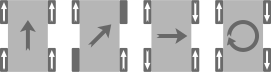
\includegraphics[width=0.8\textwidth]{graphics/mecanum_dirs.pdf}
	\caption{Podstawowe ruchy, jakie może wykonywać robot o napędzie wielokierunkowym.}
	\label{fig:mecanum_dirs}
	\end{figure} 
	
	Przykładowo, poruszając tylko przeciwległymi kołami po przekątnej, system będzie mógł poruszać po skosie, bez zmiany kąta obrotu.
	A jeśli do tego dodać obrót kół drugiej przekątnej, w odwrotnym kierunku, wtedy pojazd zacznie się poruszać w bok, pomimo faktu że koła nie są skrętne i 
	nie mogą ustawić się prosto do kierunku jazdy.
	Trasa po której porusza się robot, przy stałej prędkości kół, zawsze jest okręgiem, można uznać prostą za okrąg o nieskończonym promieniu, a punkt za okręg o zerowym.
	Wynika to z faktu, że każdy obiekt, który ma jednostajną prędkość i stały kierunek w lokalnym układzie współrzędnych, oraz prędkość kątową, będzie się poruszał po takiej krzywej.

	Podstawa ma za zadanie transportować robota manipulującego Velma, tworząc razem manipulator mobilny.
	Velma to wysoki i bardzo ciężki robot, wyposażony w dwa chwytaki na ramionach o wielu przegubach, patrz fotografia \ref{fig:velma}.
	Taka budowa wymaga szerokiej podstawy, aby zachować bezpieczną równowagę całości.
	Jeżdżąc na tej podstawie, robot może się przemieszczać i obracać w dowolnym kierunku, aby uzyskać lepszy dostęp do manipulowanych przedmiotów.
	Dodatkowe czujniki laserowe umieszczone tuż nad postawą odpowiadają za wykrywanie kolizji i lokalizację.

	\begin{figure}[H]
	\centering
	\includegraphics[width=0.5\textwidth]{graphics/velma.png}
	\caption{Robot manipulacyjny Velma.}
	\label{fig:velma}
	\end{figure} 

	Platforma jest niesymetrycznie podzielona na dwie niezależne części, przednią i tylną, w sposób pokazany na rysunku \ref{fig:base_top}.
	Przegub o jednym stopniu swobody (tzw. zawias) jest jedynym łącznikiem pomiędzy tymi dwoma fragmentami.
	Zadaniem tego przegubu jest zmniejszanie wpływu nierówności podłoża na ruch bazy, aby każde koło dociskało do podłoża z taką samą siłą, jak po drugiej stronie osi.
	Bez tego zawiasu nierówny teren uniemożliwiałby sprawne sterowanie platformą na skutek niedeterministycznego tarcia kół tej samej osi, powodując nieplanowany skręt.
	Niedeterministyczne tarcie kół jest niewykrywalne w bezpośredni sposób, jak to zostało opisane w \cite{boringbot}.

	Platforma nie jest idealnym kwadratem, jest 4 cm różnicy między szerokością, a długością robota.
	Także środki kół nie są ustawione na wierzchołkach tej figury geometrycznej.
	Szerokość jest większa, co można zobaczyć porównując widok z prawej strony \ref{fig:base_side} z widokiem z tyłu \ref{fig:base_front}.
	Dokładne wymiary są podane na rysunku \ref{fig:base_dims} i tabeli \ref{tab:dims}.

	Platforma podatna jest na losowy ruch przy rozpoczynaniu jazdy i hamowaniu.
	Jest to spowodowane tym, że asymetria rolek będzie nadawać kołom różne siły oporu, a w związku z tym różne prędkości, co w efekcie może powodować niedeterministyczny ruch.
	Należy także wziąć tutaj pod uwagę inne cechy budowy kół, jak nierówne tarcie rolek o powierzchnię \cite{braking}.

	\begin{figure}[H]
	\centering
	\includegraphics[width=0.5\textwidth]{graphics/base_top.png}
	\caption{Platforma mobilna --- widok od góry. Przegub zawiasowy łączy dwie części.}
	\label{fig:base_top}
	\end{figure} 

	\begin{figure}[H]
	\centering
	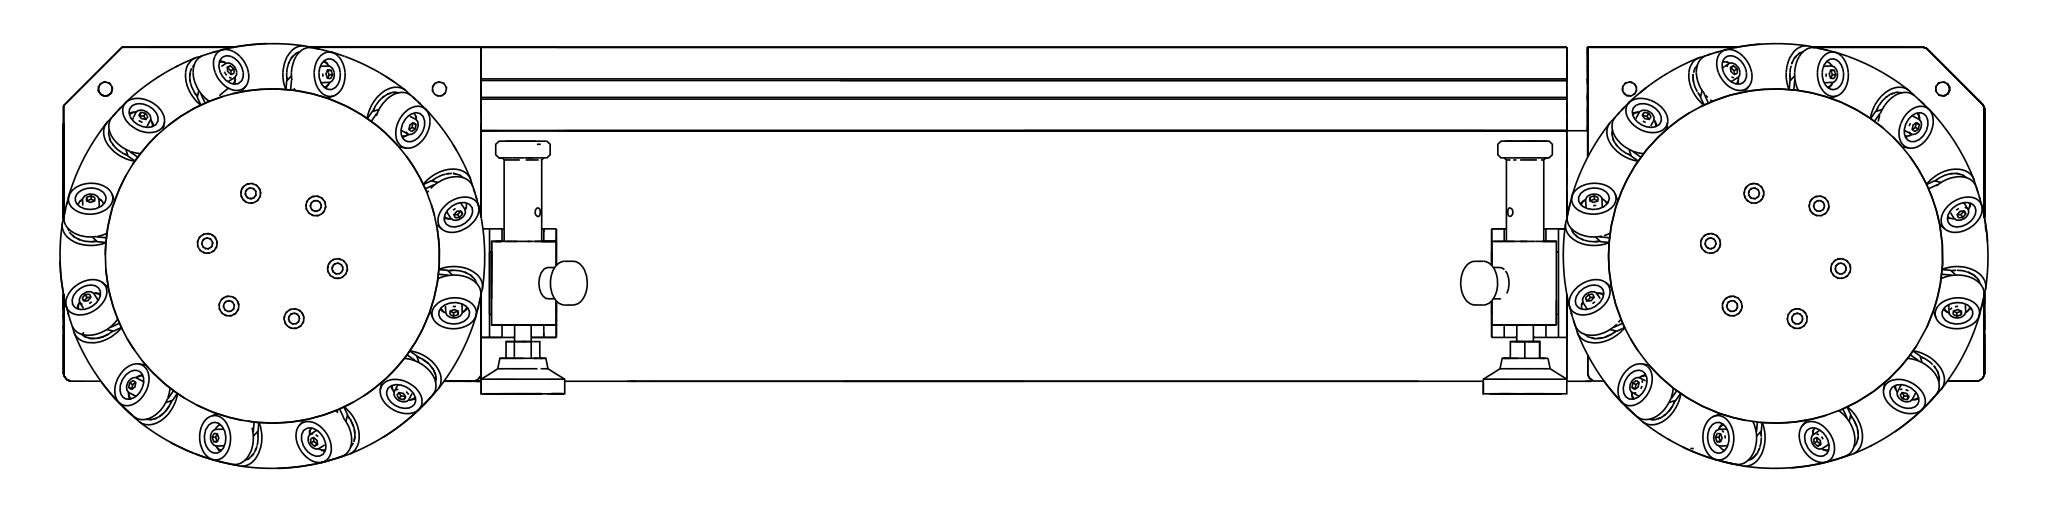
\includegraphics[width=0.5\textwidth]{graphics/base_side.pdf}
	\caption{Platforma mobilna --- widok z prawej strony.}
	\label{fig:base_side}
	\end{figure} 

	\begin{figure}[H]
	\centering
	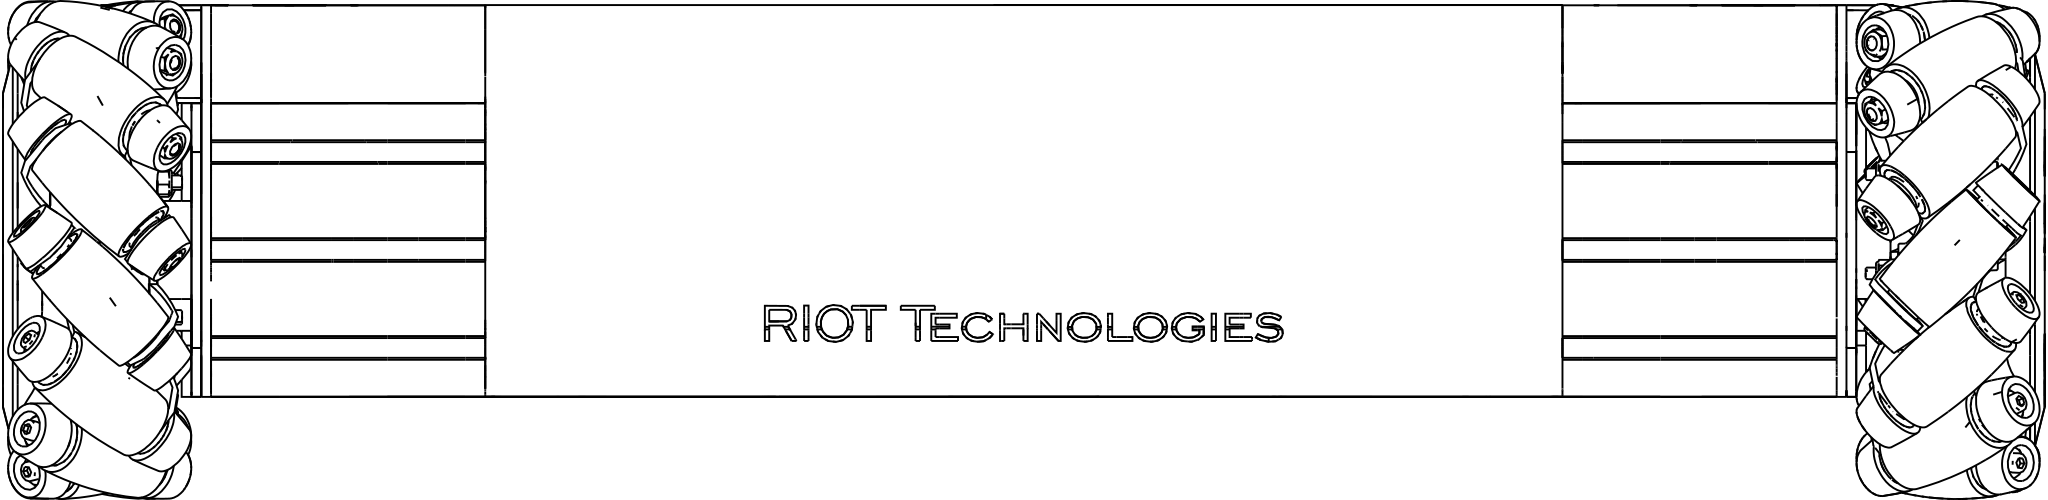
\includegraphics[width=0.5\textwidth]{graphics/base_front.pdf}
	\caption{Platforma mobilna --- widok z tyłu.}
	\label{fig:base_front}
	\end{figure} 

	Platforma posiada 3 stopnie swobody. 
	\begin{itemize}
		\item Ruch bez obrotu równolegle do osi X.
		\item Ruch bez obrotu równolegle do osi Y.
		\item Obrót w płaszczyźnie podłoża.
	\end{itemize}

\section{Koła szwedzkie}
	Koła szwedzkie, zwane także kołami Mecanum, to specjalne koła z dodatkowymi rolkami na obwodzie, ustawionymi pod kątem $45^\circ$ do osi koła.
	Rolki są pasywne i obracają się niezależnie od siebie. Każde koło ma 12 takich rolek, patrz rysunek \ref{fig:wheel}.
	W platformie ich osie ustawione są w ten sposób, że osie najwyższych, lub najniższych, rolek dwóch kół z tej samej strony robota przecinają się pod kątem prostym.
	Innymi słowy, robot ma identycznie ustawione koła na przeciwległych wierzchołkach, i razem ustawione są w kształt litery \emph{X}, patrząc na nie z góry.
	Warto pamiętać, iż oś aktualnie dolnej rolki jest prostopadła do osi górnej rolki.

	Istnieje również odwrotna odmiana ustawienia kół, w której rolki tworzą literę \emph{O}, 
	czyli oś przednia jest zamieniona z tylną, lub jakby cała platforma była odwrócona do góry nogami.
	Ten drugi sposób także pozwala na ruch wielokierunkowy, ale nie jest tak często stosowany \cite{paletobot}.

	\begin{figure}[H]
	\centering
	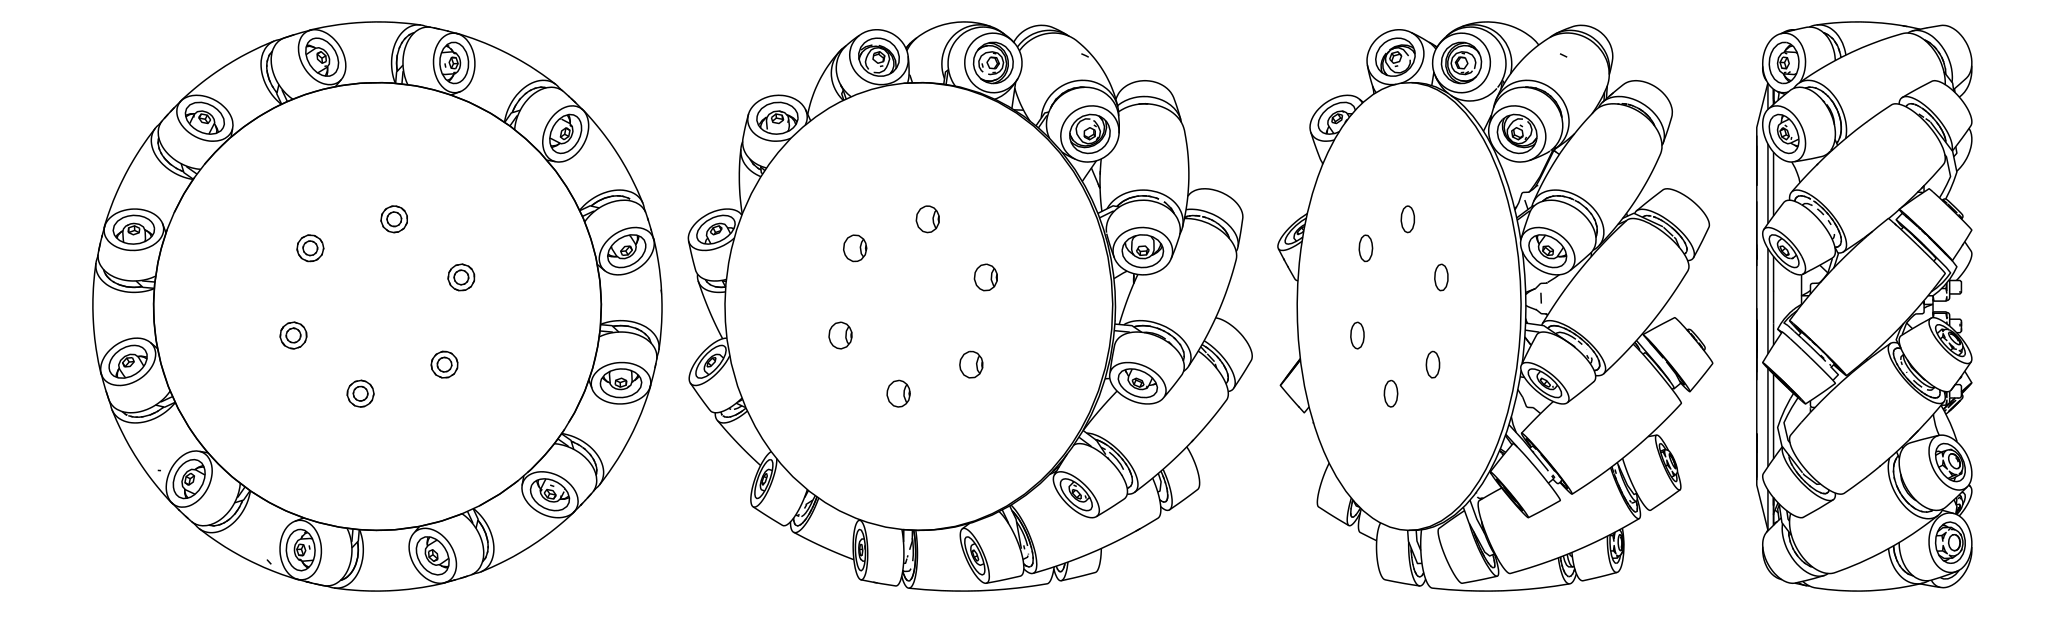
\includegraphics[width=\textwidth]{graphics/wheel.pdf}
	\caption{Widok 12 rolkowego koła szwedzkiego opisywanej platformy wielokierunkowej.}
	\label{fig:wheel}
	\end{figure} 

	Każde koło ma 3 stopnie swobody \cite{kinematic_modeling}, tak samo jak cała platforma.
	\begin{itemize}
		\item Obrót koła w osi.
		\item Rotacje pojedynczych rolek.
		\item Poślizg obrotowy w miejscu styku rolki z podłożem.
	\end{itemize}

	Na podstawie rysunku \ref{fig:wheel} widać, że krzywizna rolki jest tak ustawiona, aby punkt kontaktu rolki z podłożem w czasie obrotu płynnie przechodził na następną rolkę.
	Celem jest utrzymanie równej odległości osi od płaszczyzny podłoża.
	Nie powinno być efektu przeskoku z jednej rolki na drugą, gdyż to wprowadza nierówne tarcie, losowe poślizgi i nadmierne zużycie elementów wykonawczych.
	Kształt pojedynczej rolki zawiera się w paraboloidzie, wzory opisujące kształt rolki są złożone.
	Zazwyczaj przybliża się taką rolkę wycinkiem torusa, w celu uproszczenia produkcji \cite{rollers}.

	Istnieją także inne budowy kół, złożone z wielu małych rolek, tak aby w każdym momencie więcej jak jedna rolka dotykała podłoża.
	Można także złożyć kilka powyższych kół obok siebie w jedno koło.
	Przydatne jest to dla robotów transportujących duże masy, gdyż zmniejsza to obciążenie pojedynczych rolek.
	Niestety, taka budowa jest chroniona aktywnym patentem, więc pojedyncze koło, na które patent już wygasł, jest jedynym popularnie używanym \cite{paletobot}.

	Podstawowym problemem technologicznym koła jest nie tylko skomplikowana budowa, ale także ślizganie się rolek po powierzchni.
	Odległość osi od płaszczyzny nieznacznie zmienia się przy przenoszeniu ciężaru z rolki na rolkę, co przy dużych prędkościach powoduje drgania i jeszcze większe błędy pomiarów.
	Środkowy przegub zmniejsza ich przenoszenie na drugą część platformy.
	Poślizg kół powoduje, że enkodery nie mogą być jedynymi czujnikami służącymi do wyznaczania pozycji bazy, gdyż są zbyt mało dokładne \cite{heavy}.
	
	Dodano więc dwa czujniki laserowe, opisane dokładniej w sekcji \ref{sec:lidar}, aby program sterujący nie bazował jedynie na odometrii przy 
	wyznaczaniu sterowania. Istnieje także czujnik inercji, wykrywający zmianę rotacji i prędkość kątową robota.
	%TODO referencja

	\subsection{Działanie platformy}
	Standardowe koło, używając tarcia, przekształca prędkość kątową na liniową w płaszczyźnie obrotu. 
	Specjalne koło Mecanum ma dodatkowy wektor, równoległy do osi obrotu, 
	zatem prędkość wypadkowa jest obrócona o 45° w stosunku do wektora prędkości standardowego koła, 
	zależnie od typu koła (prawoskrętne lub lewoskrętne) i kierunku obrotu.

	\begin{figure}[H]
	\centering
	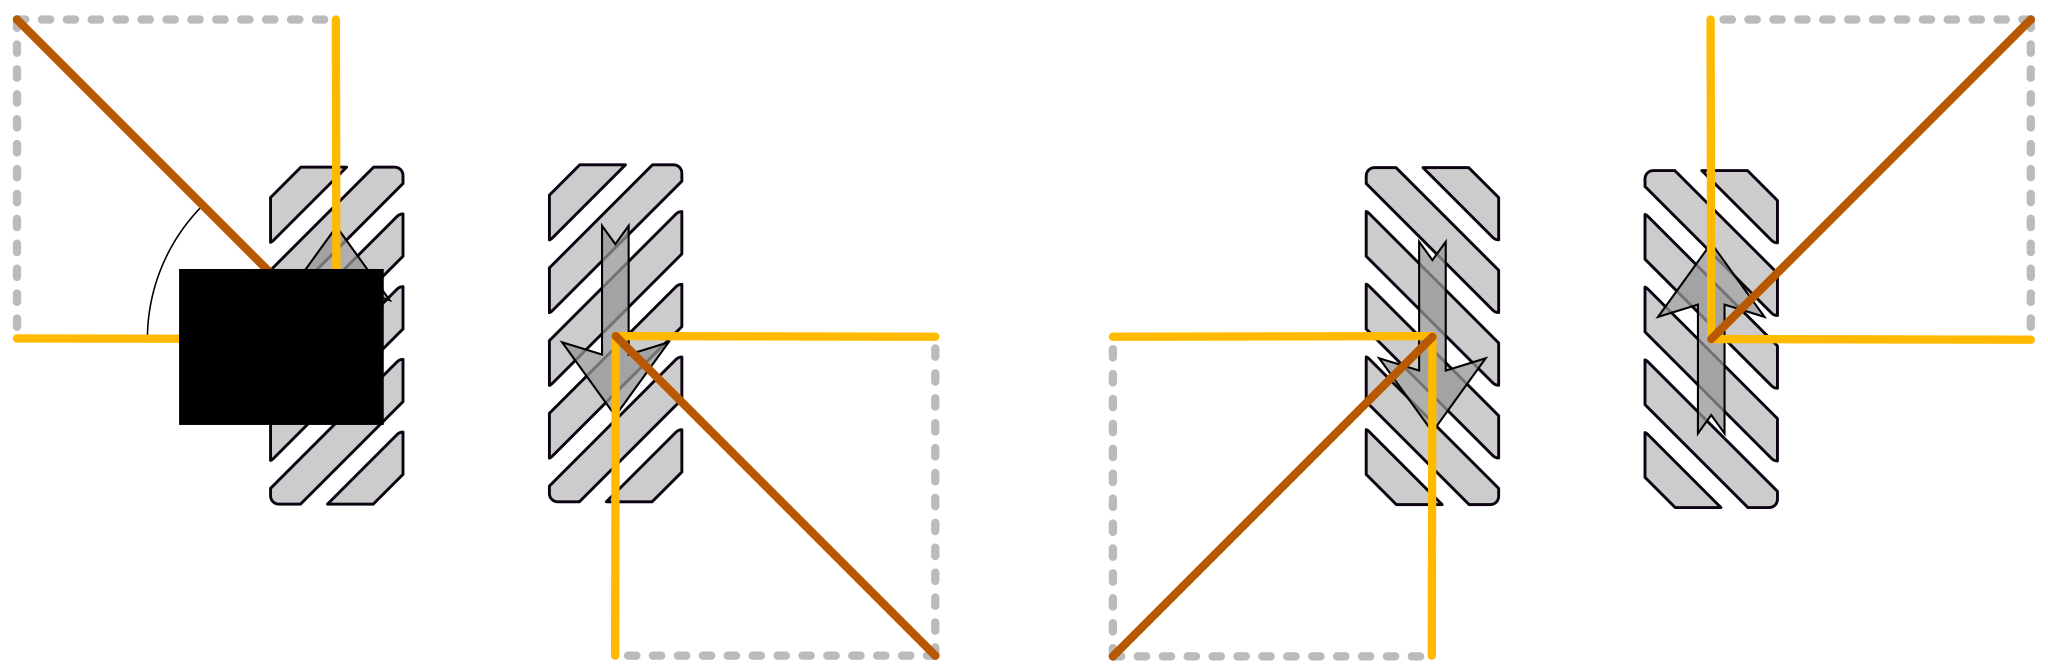
\includegraphics[width=\textwidth]{graphics/vectors.pdf}
	\caption{Wektory składowe i wypadkowe koła widzianego z góry.}
	\label{fig:wheel_vectors}
	\end{figure} 

	Ustawiając te koła w odpowiedni, opisany wcześniej na obrazku \ref{fig:base_top}, sposób, można wywołać odpowiednie znoszenie się składowych prędkości,
	a w efekcie pozwolić robotowi na poruszanie się w kierunkach nieosiągalnych dla pojazdów o standardowych kołach.
	Warto nałożyć te składowe na wcześniejszy rysunek \ref{fig:mecanum_dirs}, aby dokładniej zobaczyć, 
	dlaczego koła nadają platformie daną prędkość wypadkową przy odpowiednim obrocie kół.

	\begin{figure}[H]
	\centering
	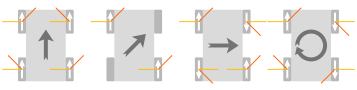
\includegraphics[width=\textwidth]{graphics/mecanum_dirs_vect.pdf}
	\caption{Ruchy platformy widzianej z góry, z nałożonymi składowymi wektorów prędkości. Ciemniejszym kolorem zaznaczono znoszące się składowe.}
	\label{fig:mecanum_dirs_vect}
	\end{figure} 

	Warto rozpatrzyć każdy przypadek. Platforma posiada jedną płaszczyznę symetrii, ze względu na asymetryczny przegub.
	\begin{enumerate}
		\item Wektory o kierunku prostopadłym do pionowej płaszczyzny symetrii urządzenia znoszą się, pomimo że mają przeciwne zwroty na przedniej i tylnej parze kół.
		Pozostają jedynie składowe równoległe do płaszczyzny symetrii, które powodują prostoliniowy ruch naprzód.
		\item Dwa koła nie obracają się. Nie jest to ruch pasywny, gdyż taki wprowadzałby nieprzewidywane poślizgi, a aktywne hamowanie.
		Wektory się nie znoszą i platforma wykonuje ruch pod kątem 45° do płaszczyzny symetrii.
		\item Ruch podobny jest do przypadku 1. Tutaj również wektory znoszą się parami, jednak tym razem na prawych kołach i lewych. 
		Pozostają składowe prostopadłe do płaszczyzny symetrii.
		\item Prędkość kątowa powstaje, gdy wypadkowa kół po jednej stronie platformy znosi się z wypadkową po drugiej stronie.
	\end{enumerate}

	Warto nadmienić, że gdy wypadkowy wektor prędkości koła jest prostopadły do osi koła, to jest gdy
	koło porusza się zgodnie z kierunkiem obrotu, w idealnym przypadku rolki nie obracają się.
	Inaczej mówiąc, rolka będzie się obracać tym mocniej, im bardziej ruch koła wymuszany jest równolegle do osi koła, 
	czy to na skutek znoszenia się wektorów, czy oporu przeszkody.
	
	Przykładowo, przy ruchu naprzód rolki koła się nie obracają, lecz przy ruchu w bok biorą aktywny udział.
	Ma to wpływ na zużywanie się tych elementów, nie tylko z punktu widzenia ilości obrotów danej rolki na pokonanym dystansie, 
	ale także sposobu w jaki wymuszany jest jej ruch.
	Rolki robota przy jeździe zawsze obracają się szarpanym ruchem w obie strony, ze względu na poślizgi od innych kół, 
	niejednostajne tarcie piast wszystkich rolek, czy różnice terenu. 
	Zatem przejazd przykładowego odcinka, przy platformie ustawionej przodem do kierunku jazdy, lub bokiem, będzie w różnym stopniu i w różny sposób zużywał elementy wykonawcze robota.
	To, jak dokładnie zużywają się przeguby i jaki styl jazdy opłaca się zastosować, aby zminimalizować uszkodzenia elementów jest dużą, odrębną dziedziną nauki.
	Odpowiednio skomplikowany algorytm sterowania może brać pod uwagę tą mechanikę kół.

\section{Czujnik laserowy}
	\label{sec:lidar}
	Program sterujący platformą nie jest w stanie dokładnie określić pozycji robota, bazując jedynie na odometrii.
	Potrzebny jest zatem czujnik laserowy.
	Platforma wyposażona jest w dwa, dwuwymiarowe czujniki typu LiDAR firmy SICK.
	LiDAR to zbitek wyrazów \emph{light} i \emph{radar}, chociaż skrót może być rozwinięty w różne słowa.

	\begin{figure}[H]
	\centering
	\includegraphics[width=0.5\textwidth]{graphics/sensor.png}
	\caption{Czujnik laserowy SICK LMS100-10000.}
	\label{fig:sensor}
	\end{figure} 

	\subsection{Zasada działania}
		Wszystkie czujniki tego typu mają bardzo podobną zasadę działania.
		W środku urządzenia znajduje się obrotowe lusterko, zwrócone pod kątem 45° do osi obrotu.
		Równolegle do osi jego obrotu znajduje się laser, który emituje pulsacyjną wiązkę podczerwonego promienia co pewien okres czasu.
		Emitowanie stałego promienia może być niebezpieczne dla wzroku obsługujących go ludzi.
		Aktualna pozycja lusterka jest wykrywana przez enkoder.
		Obok lasera jest czujnik, który bada wysłane przez laser, odbite od lusterka, obiektu i ponownie lusterka, światło.

		Na koniec, algorytm we wbudowanym mikrokontrolerze ustala kąt i odległość czujnika od wykrytego obiektu.
		Odpowiada także za usunięcie szumu i ewentualnych odbić promienia.
		Komunikacja z urządzeniem może odbywać się za pomocą różnych interfejsów sieciowych, zazwyczaj w architekturze typu master-slave.
		W przypadku tej platformy na obecny czas jest to Ethernet.
		
		Skośna szyba, będąca wycinkiem powierzchni stożka, zabezpiecza wnętrze przed zanieczyszczeniami, jej kształt niweluje ewentualne odbicia lasera, emitowanego poziomo ze środka.
		W niektórych czujnikach montuje się także szereg dodatkowych diod podczerwieni na obrębie szyby, skierowanych w górę, lub w dół, oraz czujniki/reflektory z drugiej strony.
		Pozwala to na wykrycie stopnia zanieczyszczenia szyby, aby powiadomić użytkownika o potrzebie wyczyszczenia urządzenia.

	\subsection{Komunikacja}
		Wysyłając do czujnika odpowiedni ciąg bajtów, można ustawić jego tryb działania, odpytać o zebrane dane, czy wykryć konfigurację i stan.

		W przypadku tej platformy, komunikacja odbywa się poprzez interfejsy EtherCAT i Ethernet.
		EtherCAT to sposób komunikacji urządzeń po kablu Ethernetowym, w trybie \emph{master}-\emph{slave}, przy zachowaniu sztywnych ram czasowych. 
		\emph{Master} wysyła pakiet do podłączonych szeregowo urządzeń \emph{slave}, które przekazują go przez siebie i w razie potrzeby modyfikują dane w locie.
		
		Program odbierający dane od czujnika komunikuje się bezpośrednio z urządzeniem, które zwraca pakiety zawierające pomiary z ostatniego obrotu czujnika, oraz dodatkowe dane 
		opisujące sam pomiar, takie jak czas, początkowy kąt pomiaru, czy tryb pacy.
		Dokładne pola w pakiecie i cechy czujnika dostępne są na stronie producenta \cite{sick_website}.

		Urządzenie wspiera uwierzytelnianie przez hasło, wgrywanie nowego oprogramowania,
		ustawienia czasu, oraz zmianę różnych parametrów działania.

	\subsection{Podstawowe cechy}
		Czujnik składa się z dwóch części, głównego trzonu, oraz nakładki.
		Połączenie tych elementów powoduje, że jego zakres pomiaru posiada martwy kąt.
		Przedstawia to dobrze grafika producenta \ref{fig:lidar}.
		\begin{figure}[H]
		\centering
		\includegraphics[width=0.6\textwidth]{graphics/sick.png}
		\caption{Wykres producenta dotyczący zasięgu czujnika.}
		\label{fig:lidar}
		\end{figure} 
		
		\begin{table}
		\centering
		\begin{tabular}{l r}
		Cecha & Wartość \\
		\hline
		Kąt pracy & 270\textdegree \\
		Długość fali światła lasera & 905 nm (podczerwień) \\
		Częstotliwości skanowania & 25 Hz / 50 Hz \\
		Maksymalna odległość obiektu & $\approx$ 20 m \\
		Rozdzielczość kątowa & $0,25 \degree$ / $0,5 \degree $ \\
		Systematyczny błąd pomiarowy & $\pm 0,03$ m \\
		Przypadkowy błąd odległości & $0,012$ m \\
		\end{tabular}
		\caption{Podstawowe cechy czujnika laserowego.}
		\label{tab:lidar}
		\end{table}
		Na podstawie tych danych można obliczyć, że w jednym przebiegu po całym zakresie kątowym urządzenia, 
		emitowane jest około 1080, lub 540 impulsów (w zależności od trybu działania).
		Taka ilość promieni wymagana jest w symulacji, aby wiernie odwzorować urządzenie.

\chapter{Środowiska programistyczne} 
\label{sec:tools}
W tym rozdziale opisane są narzędzia użyte do wykonania zadania.

Środowisko symulacji składa się z maszyny symulującej fizykę, odpowiedzialnej za obliczenia fizyczne, a także API do obsługi całej symulacji.
Zaawansowana maszyna symulacyjna powinna dobrze obsługiwać tarcia, więzy na ruch obiektów, przyłożone siły, materiały fizyczne dla określania tarcia i sprężystości obiektów, 
oraz wszystko to, co potrzebne do jak najwierniejszego odtworzenia zachowania rzeczywistego obiektu.

Na rynku jest wiele różnych maszyn, zarówno do symulacji w czasie rzeczywistym, jak i do wyznaczania pozycji obiektów po długich obliczeniach.
Istnieją technologie otwartoźródłowe, inne są własnościowe. Mogą używać tylko procesora, lub też być wspomagane przez kartę graficzną (na przykład \emph{PhysiX}).
Niektóre maszyny symulują, prócz zderzeń obiektów, także rozpływ cieczy, dymy, płótna, ciała sprężyste i strukturę wewnętrzną brył, 
lecz te funkcjonalności nie są potrzebne dla symulacji opisywanej platformy. Nazywa się je czasami ,,silnikami symulacji fizyki'', co jest bezpośrednim tłumaczeniem nazwy
\emph{physics engine} z języka angielskiego.

\section{ROS}
	ROS jest skrótem od \emph{Robot Operating System}, lecz jego nazwa jest myląca.
	Nie jest to system operacyjny, lecz obszerna platforma programistyczna (\emph{framework}), zawierająca odpowiednie biblioteki i narzędzia do tworzenia programów sterujących.
	ROS stara się w łatwy sposób dostarczyć wszystko, co potrzebne do budowy logiki aplikacji sterowania.
	Są tu algorytmy wyznaczania tras, budowy map, manipulowania robotycznymi ramionami itp. 
	Platforma programistyczna do pobrania jest z \cite{ros_website}.

	Twórcy zachęcają, aby uzupełniać brakujące moduły swoimi własnymi, a potem dzielić się nimi z resztą programistów.
	Na ich stronie internetowej znajduje się obszerna baza danych różnych komponentów, do używania we własnych systemach.

	Programy dla ROS pisze się w C++, lub Pythonie i integruje z robotem za pomocą kilku gotowych struktur kolejek wiadomości.
	Platforma ta także posiada moduły do wizualizacji odbieranych danych w formie graficznej.

	Działanie systemu jest oparte o pakiety.
	Każdy taki komponent jest katalogiem zawierającym w sobie pliki opisujące jego parametry i skrypty CMake, używane do kompilacji.
	Pakiet może być programem wykonywalnym, danymi, definicjami, lub zestawem plików.
	W symulacji opisywanej platformy, modele są plikami i programami, łączonymi razem we wspólnym pakiecie, ładowanym do pakietu programu wykonywalnego.
	Jest to dokładnie opisane w rozdziale \ref{sec:components}.
	Pakiety mogą być zależne od siebie, ale nigdy nie wskazują nawzajem swoich bezpośrednich ścieżek.

	Globalny skrypt kompilacji ROSa dba o odpowiednie podawanie ścieżek, kolejność kompilacji programów i załączanie nazw.
	Na przykład, jeśli pakiet wymaga pliku nagłówkowego, generowanego przez kompilację innego pakietu, załącza go w kodzie tak, jakby był systemowy.
	Skrypt CMake zadba o wywołanie kompilatora z odpowiednimi argumentami.

	Komunikacja między programami odbywa się w sposób ciągły przez kolejki wiadomości, lub pojedyncze asynchroniczne wywołania, zwracające wynik.
	Program może nadawać strumień wiadomości, ale niekoniecznie musi istnieć w tym czasie odbiornik.
	Można buforować wiadomości, podglądać strumienie, tworzyć wykresy z danych, podłączać nadajnik do kilku odbiorników, podglądać graf zależności itp.
	Do wszystkiego służy bogaty zestaw komend i wbudowanych narzędzi.

	Instalacja programu na systemie operacyjnym jest złożona.
	Z wyjątkiem odpowiednich wersji Ubuntu, nie ma łatwego sposobu na instalację go na innych systemach.
	Na przeszkodzie stoją błędy kompilacji dla nowszych wersji kompilatorów, zależności od dokładnych wersji zewnętrznych bibliotek i 
	inne problemy w czasie wykonywania, jak naruszenie ochrony pamięci. 
	Instalacja alternatywnych pakietów i ręczna kompilacja niektórych części nie działa we wszystkich przypadkach.

	Rozwiązaniem tego problemu jest instalacja tej platformy programistycznej na maszynie wirtualnej, lub na systemie uruchamianym z dysku zewnętrznego. 
	Najnowszą wersją ROSa jest \emph{Lunar Loggerhead} z maja 2017, jednak nie jest to wersja długiego wsparcia, a co za tym idzie, nie posiada wszystkich
	pakietów zewnętrznych twórców, potrzebnych przy wizualizacji symulacji.
	Odpowiedniejszą wersją jest \emph{Kinetic Kame} z marca 2016 roku, o bardzo dobrym wsparciu.
	Pakiety składające się na system ROS nadal są regularnie aktualizowane, lecz nie zawierają nowych funkcjonalności, a jedynie poprawki błędów.
	Główny symulator fizyki, najważniejszy program, jest w tej samej wersji w obu dystrybucjach.

	Uruchomienie platformy programistycznej na systemie wymaga wielu dodatkowych komend inicjalizujących, 
	a także dopisywania do tworzonych projektów licznych plików konfiguracyjnych za pomocą dostarczonych skryptów.
	Używanie modułów z linii poleceń wymaga ustawienia kilku zmiennych systemowych, poprzez wczytywanie skryptów.
	Użycie niektórych funkcji ROS wymaga uruchomionego demona serwera w tle.

	Ogólnie instalacja i używanie ROS na systemie zostawia dużo różnorodnych plików w katalogu domowym, co może nie być wskazane na codziennym systemie operacyjnym.
	Z drugiej jednak strony, wirtualizacja systemu operacyjnego z ROS bardzo ogranicza dostępną moc obliczeniową, potrzebną takim programom w dużych ilościach.

\section{Gazebo}
	Program do pobrania z \cite{gazebo_website}. 
	Ten symulator graficzny jest dość prosty w obsłudze, skupia się na symulowaniu podanych danych, a nie na możliwości ich łatwego przygotowania.
	To znaczy, działa na podstawie manualnie napisanych plików konfiguracyjnych.
	Zazwyczaj używany w trybie wsadowym, uruchamiany z argumentami z linii poleceń i plikiem \texttt{world}, opisującym symulację.
	Plik ten zawiera nazwy i ścieżki umieszczanych w symulacji modeli i wtyczek.
	Z tego powodu interfejs graficzny jest dość ubogi.

	Program przeprowadza symulację podanych modeli, używając jednego z czterech popularnych maszyn symulacyjnych: ODE, Bullet, Simbody lub DART.
	Wszystkie te projekty są wolnym oprogramowaniem i używane są także w innych programach, na przykład w edytorze Blender.

	Symulator oprócz tego ma wbudowany edytor modeli, w którym można składać i ustawiać odpowiednie obiekty razem w przestrzeni trójwymiarowej
	i generować powyższy plik.
	Edytor budynków pozwala na stawianie wirtualnych ścian, korytarzy, drzwi i ogólnego otoczenia w którym roboty mogą pracować i być symulowane.
	Funkcjonalność tych edytorów jest bardzo ograniczona, brak jest tak podstawowych funkcji, jak cofanie ruchu.
	Dlatego lepiej jest zdefiniować model we wczytywanym pliku tekstowym.
	Również tworząc modele poza edytorem, posiada się nad nimi większą kontrolę, a parametry obiektów da się ustawiać z dowolną dokładnością.

	Gazebo przyjmuje modele w specjalnym formacie SDF. Jest to ustandaryzowany, zdefiniowany zewnętrznie format, do opisywania budowy robotów i czujników.
	Dzięki temu plik SDF może być użyty w innej symulacji, w innym programie, pod warunkiem przestrzegania standardu.
	Składnia jest standardowym XML, co znaczy, że może być tworzona na każdym edytorze tekstowym.

	Wtyczka do sterowania modelem jest skompilowaną biblioteką, dołączaną na starcie programu.
	Tworzy się ją w C++, lub Pythonie, jako klasę dziedziczącą po abstrakcyjnej klasie dostarczonej przez Gazebo.
	Dzięki temu może korzystać ze wszystkich funkcjonalności systemu operacyjnego, jak na przykład komunikacja za pomocą pamięci współdzielonej.
	Gazebo dostarcza także swój własny mechanizm kolejek wiadomości, który sprawdza się w jednolitej komunikacji z zewnętrznymi programami, korzystającymi z bibliotek 
	dostarczonych przez Gazebo, jednak jest niezależny od podobnej mechaniki ROSa.

	Program jest w pełni wspierany na dystrybucji GNU/Linuksa Ubuntu ale bez problemu można go także skompilować pod inne systemy.
	Interfejs jest dopracowany i przestrzega wielu ustawień systemowych, na przykład takich jak DPI, lecz nie korzysta z dedykowanych bibliotek do tworzenia 
	interfejsów typu Qt, lub GTK.
	Uruchamianie programu jest proste i nie wymaga dodatkowych ustawień, wywoływania skryptów inicjalizujących, 
	tworzenia odpowiednich katalogów, czy definiowania zmiennych systemowych.
	Podobnie jak inne programy, tworzy ukryty katalog w katalogu domowym użytkownika, gdzie składuje wszystkie modele i logi.

	Gazebo może także być składnikiem systemu ROS, kod źródłowy jest dzielony w ramach wspólnej organizacji.
	Chociaż różne osoby odpowiadają za rozwój tych oprogramowań,
	kolejne wersje Gazebo są powiązane z kolejnymi wersjami ROSa, nie można użyć przestarzałej wersji Gazebo z nowszym ROSem i odwrotnie.
	Symulator można zainstalować osobno, lub jako jeden z pakietów ROSa.
	Jednakże, ze względu na chęć zachowania wysokiej kompatybilności pakietów ROSa, to nienajnowsza wersja Gazebo jest dostarczana z ROSem.

\section{V-Rep}
	Program do pobrania z \cite{vrep_website}. Duże i skomplikowane środowisko, reklamujące się wieloma zaawansowanymi mechanizmami i funkcjami.
	Pomimo otwartego kodu, użycie komercyjne jest płatne. Dla zastosowań akademickich program jest rozdawany bez opłat.
	Bogaty interfejs graficzny zakłada budowę i symulację wszystkiego w tym jednym programie.

	Używa dwóch z maszyn symulacyjnych Gazebo, czyli ODE i Bullet, oraz dodatkowo Vortex i Newton. Z tej czwórki tylko Vortex ma zamknięty kod.

	Głównym mankamentem programu jest zapisywanie utworzonych w systemie modeli.
	Program tworzy drzewiastą strukturę modelu, w pliku binarnym własnego formatu, co uniemożliwia edycję i wizualizację modelu bez uruchamiania całego programu 
	i importowania modelu do symulacji.
	Brak przenośności, czy wsparcia systemu kontroli wersji dla takich nietekstowych plików także jest problemem.

	Pisanie wtyczek najczęściej odbywa się w Lua. Są też jednak dostępne inne języki, jak C, Matlab, Java itp.
	Komunikacja z innymi programami odbywa się poprzez specjalne wtyczki do środowiska.
	API pozwala stworzyć mały, wbudowany interfejs graficzny do sterowania symulacją poprzez przyciski i suwaki.

	Ze strony producenta pobrać można gotowe archiwum z programem, który nie wymaga żadnej instalacji i posiada wszystkie potrzebne zasoby do pracy i nauki, 
	jak przykładowe modele istniejących komercyjnych robotów.
	Program działa w trzech najpopularniejszych systemach operacyjnych --- Windows, Linux i OS X.

\section{Narzędzia}
	Do tworzenia oprogramowania na systemach Unixowych można użyć dowolnych edytorów, gdyż standardowo wszystko jest potem kompilowane za pomocą narzędzi wiersza poleceń i skryptów.
	Jednak warto sobie ułatwić pracę zaawansowanymi środowiskami graficznymi.
	\begin{description}
	\item[CMake] to popularny i używany przez ROS i Gazebo system budowy kodu. Program tworzy na podstawie swoich plików konfiguracyjnych plik \texttt{makefile} do kompilacji źródeł i łączenia bibliotek.
	\item[GCC] będzie użyty do kompilacji, gdyż jest to najpopularniejszy tego typu program używany w GNU/Linux. Same symulatory zostały w nim skompilowane.
	\item[KDevelop] jest graficznym edytorem tekstowym i nadaje się do pisania kompilowalnego kodu wtyczek. Można podłączyć je pod komendę \texttt{make} i korzystać z mechanizmów interpretacji błędnych linii kodu, graficznego debugowania i podobnych.
	\item[Bash] będący bardzo popularnym językiem skryptowym nadaje się do automatyzacji pracy i uruchamiania testów w kontrolowany i prosty sposób.
	Uniwersalne narzędzie pomagające w wielu miejscach.
	\item[Git] jest narzędziem kontroli wersji, używanym przy bardzo wielu projektach informatycznych. Pozwala na łatwe umieszczenie kodu w usłudze GitHub.
	\item[Gnuplot] służy do generowania wykresów z danych, zapisanych w pliku tekstowym.
	\item[Dia] to graficzny edytor do tworzenia diagramów UML.
	\end{description}



\chapter{Środowisko symulacyjne}
\label{sec:model}
W tym rozdziale opisane są stworzone składniki systemu, czyli modele dynamiczne i kinematyczne, modele czujników, oraz pakiety wspomagające testowanie.

Aby uruchomić symulację, nie wystarczy uruchomienie symulatora z modelami, należy zadbać także o odpowiednie przekazywanie informacji do i z symulowanych obiektów.
Wskazane jest przetestować modele, czy zachowują się poprawnie w prostych scenariuszach testowych, tak samo, jak testować się będzie program sterujący na modelu.
Do tego potrzebne są programy wspomagające, które łączy się w różne konfiguracje, w zależności od scenariusza testowego.
Ze względu na niezależność pakietów od siebie, można ich także użyć przy komunikacji z rzeczywistym robotem.

Środowisko symulacyjne składa się z kilku odrębnych pakietów, które komunikują się ze sobą poprzez specjalne interfejsy, wykorzystujące kolejki wiadomości.
Taka implementacja komunikacji pozwala zmieniać i reimplementować poszczególne elementy, używać różnych języków programowania, oraz
zachowywać jednolitą komunikację między składnikami i nie tracąc na kompatybilności między pakietami.
Możliwe jest także przesyłanie wiadomości przez sieć, co pozwala na rozproszenie systemu.

Niektóre typy wiadomości posiadają wbudowany nagłówek, inne istnieją w dwóch wersjach, z nagłówkiem i bez. 
Dopisek \texttt{Stamped} określa istnienie tej dodatkowej informacji.
Nagłówek ma trzy pola:
\begin{itemize}
	\item Numer sekwencyjny, zwiększany przez program wysyłający po każdej wysłanej wiadomości.
	\item Czas nadania wiadomości, z dokładnością do nanosekund.
	\item Identyfikator macierzy przekształcenia jednorodnego, według której podano dane, ta funkcjonalność została opisana dokładniej w sekcji \ref{sec:frames}.
\end{itemize}

\begin{table}
	\centering
	\begin{tabular}{l r}
		Typ & Opis \\
		\hline
		\texttt{omnivelma\_msgs/Encoders} & Prędkości i pozycje kół z enkodera. \\
		\texttt{omnivelma\_msgs/Vels} & Prędkości kół. \\
		\texttt{omnivelma\_msgs/SetFriction} & Nadanie tarcia elementowi modelu. \\
		\texttt{omnivelma\_msgs/SetInertia} & Nadanie mas i momentu bezwładności obiektowi. \\
		\texttt{geometry\_msgs/Pose} & Pozycja obiektu w przestrzeni kartezjańskiej. \\
		\texttt{geometry\_msgs/Twist} & Prędkość względna obiektu. \\
		\texttt{sensor\_msgs/LaserScan} & Jedno skanowanie skanera laserowego. \\
		\texttt{omnivelma\_msgs/Relative} & Odległość i kąt pomiędzy obiektami. \\
		\texttt{nav\_msgs/Odometry} & Pozycja obiektu z macierzą kowariancji. \\
		\texttt{sensor\_msgs/Imu} & Dane generowane przez jednostkę inercyjną. \\
	\end{tabular}
	\caption{Typy wiadomości przekazywanych pomiędzy pakietami.}
	\label{tab:messages}
\end{table}

Pakiety można podzielić na trzy typy:
\begin{itemize}
	\item Generujące dane.
	\item Przekazujące i modyfikujące dane.
	\item Zbierające dane.
\end{itemize}
Poniżej, każdy pakiet opisany jest bardziej szczegółowo, wraz z jego interfejsem.

W trakcie testowania symulatora, podłączenie pakietów będzie wyglądać następująco:
\begin{figure}[H]
	\centering
	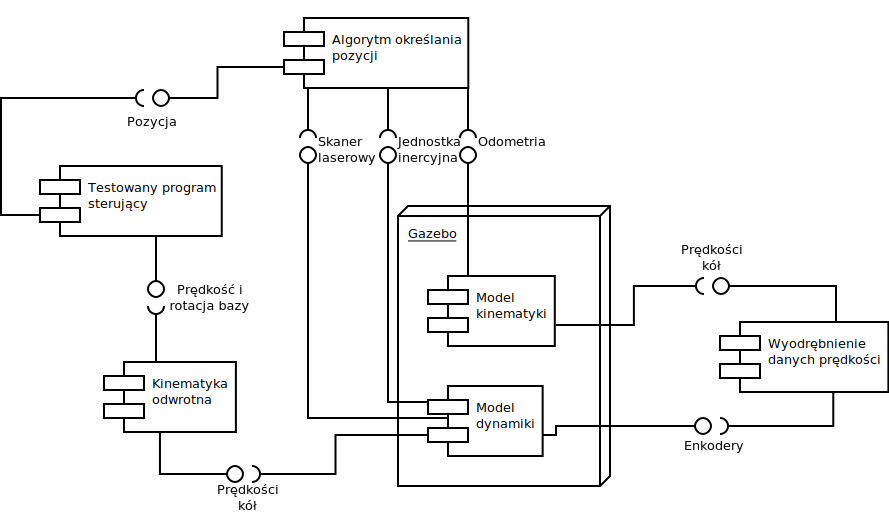
\includegraphics[width=\textwidth]{uml/final.pdf}
	\caption{Komunikacja podstawowych pakietów systemu w trakcie testowania programu sterującego.}
\end{figure}

Ważną rolę odgrywa tutaj algorytm określania pozycji, bazujący na odometrii, jednostce inercyjnej i danych ze skanera laserowego.
Odometria jest generowana za pomocą modelu kinematycznego, sterowanego danymi z enkoderów modelu dynamicznego.
Sam model dynamiczny sterowany jest pośrednio przez program, który generuje zadane prędkości i obrót robota.
W uproszczeniu: program sterujący wysyła sterowanie do modelu, bazując na jego pozycji, określonej z danych generowanych przez modele czujników.

W każdym miejscu przepływu danych można zebrać i zwizualizować przesyłane wartości.
Program sterujący może także korzystać ze skanerów laserowych w celu wykrycia przeszkody, nie tylko w celu określenia pozycji.
Bardziej zaawansowany program sterujący mógłby generować zadane prędkości kół bezpośrednio, nie bazować na modelu kinematyki odwrotnej.

\section{Zapis agentowy}
	Aby zachować kompatybilność programu sterującego platformy mobilnej z jej modelem, należy stworzyć efektory i receptory wirtualne, do których 
	program sterujący będzie wysyłał i z których będzie odbierał dane. 
	Te wirtualne byty będą dalej przekazywać informacje zarówno do modeli, jak i do robota w taki sposób, że
	główny program sterujący nie będzie miał żadnej informacji o tym, do czego jest podłączony. 
	
	\begin{figure}[H]
		\centering
		\includegraphics[width=0.8\textwidth]{graphics/agent.pdf}
		\caption{Struktura agenta upostaciowionego.}
		\label{fig:agent}
	\end{figure} 

	Można to przedstawić za pomocą zapisu agentowego, rysunek \ref{fig:agent}.
	Agent upostaciowiony składa się z kilku modułów, komunikujących się ze sobą za pomocą różnych interfejsów.

	Nadrzędnym modułem jest układ sterowania, który na podstawie odczytów z czujników generuje sterowanie dla efektorów.
	Ważne jest, aby komunikacja z rzeczywistymi urządzeniami była identyczna, jak z ich modelami, dzięki czemu taki system będzie przenośny i niezależny od implementacji modelu.

	Efektor rzeczywisty, na przykład serwomotor, jest sterowany za pomocą efektora wirtualnego, który zamienia wyjście układu sterowania na sygnały sterujące dla silnika napędowego.
	Przykładowo, zmienia odebraną liczbę, oznaczającą zadaną prędkość, na odpowiednie napięcie na wyjściu układu sterującego.

	Zamodelowany efektor symulowany również przyjmuje te same sygnały do układu sterowania, co efektor rzeczywisty, 
	lecz nie zamienia ich na sygnały sterujące, a wywołuje odpowiednie funkcje maszyny symulacyjnej, nadające siły i prędkości obiektom w przestrzeni wirtualnej.

	Receptor wirtualny pobiera surowe dane z czujnika, przekształca na odpowiedni format, usuwa błędy i szum tak, aby program sterujący mógł wykorzystać te dane w prosty sposób. 
	Doskonałym przykładem jest tutaj urządzenie Kinect (widoczne na robocie Velma na rysunku \ref{fig:velma}), w którym to zachodzi odczytanie obrazu z kilku kamer.
	Następnie obraz przesyłany jest do komputera, w którym sterowniki interpretują dane, usuwając błędy, tworzą mapę głębokości, wykrywają szkielety i sylwetki osób.
	Te dane mogą być wykorzystane łatwo w grach i programach sterujących.

	Modelowanie receptora, tak jak w przypadku efektora, polega na wygenerowaniu odpowiednich danych, używając odpowiednich funkcji w przestrzeni wirtualnej.
	Mogą one polegać na emitowaniu półprostych, symulujących laser, lub wręcz renderowaniu obiektów, aby uzyskać obraz z wirtualnej kamery.
	Receptor symulowany ma pełną wiedzę o symulowanym świecie, dokładne pozycje i prędkości wszystkich obiektów, dane o kolizjach itp. 
	Pozwala to na łatwe symulowanie receptorów nie mogących mieć odwzorowania w rzeczywistości, co przydatne jest w pierwszych stadiach testowania i wyznaczaniu statystyk.
	Takim przykładem jest model czujnika dokładnej pozycji, rotacji i prędkości w kartezjańskim układzie współrzędnych. 
	Czujniki typu GPS, lub żyroskopy nie generują tak dokładnych pomiarów.


\section{Model kinematyczny}
	\label{sec:pseudovelma}
	Kinematyka opisuje ruch obiektów bez rozważania sił powodujących ten ruch.
	Nie uwzględnia się przy opisie ruchu takich czynników, jak masa, moment bezwładności, czy siły.
	
	Model kinematyki określa równania prostego zadania kinematyki. 
	Rozwiązanie tego zadania polega na obliczeniu prędkości liniowej i kątowej bazy mobilnej na podstawie aktualnych prędkości kół.
	Symulator pozwala również na całkowanie tych prędkości, aby uzyskać aktualną pozycję platformy, z dokładnością do pozycji startowej.
	
	Równania modelu kinematyki najwygodniej przedstawić w postaci macierzowej, podobnej do tego, jak opisano w \cite{wheels}. 
	Dokładna podstać wzoru zależy od kolejności numerowania kół i interpretacji wymiarów.
	Dla opisanego tutaj przypadku, (stałe zdefiniowane są w tabeli \ref{tab:dims}, numeracja kół jest pokazane na rysunku \ref{fig:base_dims}):
	
	\begin{equation}
	\begin{bmatrix}
	v_x \\
	v_y \\
	\omega_z \\
	\end{bmatrix}
	=
	\frac{r}{4}
	\begin{bmatrix}
	-1 & 1 & -1 & 1 \\
	1 & 1 & 1 & 1 \\
	\frac{2}{a+b} & \frac{-2}{a+b} & \frac{-2}{a+b} & \frac{2}{a+b} \\
	\end{bmatrix}
	\begin{bmatrix}
	\omega_1 \\
	\omega_2 \\
	\omega_3 \\
	\omega_4 \\
	\end{bmatrix}
	\end{equation}
	
	Uzyskane wartości należy zastosować w funkcjach symulatora, aby nadać obiektom wirtualnym odpowiednie prędkości.
	
	Sterowanie pozycją modelu kinematycznego odbywa się wyłącznie poprzez powyższy wzór, zatem w jego symulacji nie uczestniczy maszyna symulacyjna fizyki.
	Ten model nie reaguje na kolizje z innymi obiektami, nie reaguje na różnicę terenu i nie używa informacji o współczynnikach tarcia materiałów.

	\subsection{Zachowanie}
		Platforma ignoruje inne obiekty znajdujące się na scenie,
		Po nadaniu stałych prędkości kół, następuje ruch zgodnie z rysunkiem \ref{fig:mecanum_dirs}.

		Program sterujący co każdy krok symulacji (okres zależy od zasobów procesorowych komputera) zwraca aktualne położenie i orientację, oraz prędkość liniową i kątową. 

\section{Model dynamiczny}
	\label{sec:omnivelma}
	Maszyna do symulacji dynamiki używa informacji o kształtach, masach i złączach pomiędzy ogniwami robota.
	Należy zatem stworzyć obiekt, złożony z modeli ogniw i samych ogniw i umieścić w symulatorze.
	Potem należy nadać obiektom odpowiednie siły, aby otrzymać wyniki przybliżone do tego, jak zachowywałaby się rzeczywista baza mobilna.

	Baza mobilna jest bryłą, na którą składają się następujące części składowe:
	\begin{itemize}
	\item Główna część korpusu.
	\item Ruchoma, mniejsza część korpusu, z przodu robota.
	\item 4 koła, 2 podłączone do głównej części korpusu, a 2 do przedniej.
	\item Po 12 rolek na każdym kole.
	\item Przegub obrotowy, łączący dwie części korpusu.
	\item 4 przeguby obrotowe z silnikami, łączące części bazy z kołami.
	\item 12 przegubów obrotowych na każdym kole, łączących koła z rolkami.
	\end{itemize}

	Jest to dość złożony obiekt do symulacji, dlatego należy dążyć do uproszczenia modelu, w celu zmniejszenia ilości obliczeń symulatora.
	Istnieje wiele podejść do stworzenia odpowiedniego modelu, na przykład jak najdokładniejsze odwzorowanie budowy platformy 
	za pomocą wzorów różniczkowych \cite{braking} \cite{modelling_ways}.
	
	\subsection{Zachowanie}
		Model reaguje na siły przyłożone do jego ogniw, porusza się, reagując na otoczenie.
		Bierze udział w kolizjach, nadaje prędkości innym obiektom.
		Współczynniki tarcia podłoża i kół mają znaczenie w symulacji.
		Powstają niedokładności wyznaczania pozycji, spowodowane dużą ilością zmiennych, uczestniczących w symulacji i precyzją symulatora.
	
\section{Model skanera laserowego}
	\label{sec:monokl}
	Symulator generuje odpowiednie dane, emitując promienie w przestrzeni wirtualnej.
	Następnie maszyna symulacyjna fizyki oblicza kolizje promieni z obiektami na scenie.
	Jest to operacja bardzo kosztowna obliczeniowo.
	
	Do położeń punków dodawany szum o rozkładzie normalnym, aby symulować błędy pomiarowe, powstałe przy odczycie odbicia lasera.
	
	Odczyt z rzeczywistego skanera pokazuje, że sztucznie wygenerowane dane są podobne do danych zebranych przez czujnik.
	Dodatkowo, wbudowany w czujnik sterownik usuwa błędy grube z pomiarów, zatem rzeczywiste dane nie posiadają ich, więc i nie jest konieczne dodawanie ich do modelu.
	
	\begin{figure}[h]
	\centering
	\includegraphics[width=\textwidth]{graphics/scan.png}
	\caption{Zrzut ekranu platformy z Gazebo i wygenerowane dane, obserwowane w Rviz.}
	\label{fig:scan}
	\end{figure}
	
\section{Model jednostki inercyjnej}
	Rzeczywisty czujnik obarczony jest bardzo dużymi błędami pomiarowymi.
	Jednakże, jego model także zwraca bardzo zaszumiony obraz.
	
\section{Model kinematyki odwrotnej}
	\label{sec:transmutator}
	Jest to model kinematyki odwrotnej, alternatywa do modelu kinematycznego, opisanego w sekcji \ref{sec:pseudovelma}, jednak działającego bez symulatora i bez możliwości 
	całkowania prędkości (i generowania danych o aktualnej pozycji).
	Całkowanie prędkości kół i tak nie ma większego sensu, ponieważ pozwoliłaby jedynie obliczyć aktualną ich pozycję.
	Z wyjątkiem porównania tych danych z danymi z enkoderów, nie ma to zastosowania.
	
	Ten pakiet przyjmuje zadaną prędkość, kierunek i obrót platformy, a zwraca prędkości kół, które powinny być nadane platformie, aby wywołać taki ruch.
	Wzory mogą być przedstawione w postaci macierzowej.
	
	\begin{equation}
	\begin{bmatrix}
	\omega_1 \\
	\omega_2 \\
	\omega_3 \\
	\omega_4 \\
	\end{bmatrix}
	=
	\frac{1}{r}
	\begin{bmatrix}
	1 & -1 & \frac{a+b}{2} \\
	1 & 1 & -\frac{a+b}{2} \\
	1 & -1 & -\frac{a+b}{2} \\
	1 & 1 & \frac{a+b}{2} \\
	\end{bmatrix}
	\begin{bmatrix}
	v_y \\
	v_x \\
	\omega_z \\
	\end{bmatrix}
	\end{equation}
	
	Stałe, użyte we wzorze zdefiniowane są w tabeli \ref{tab:dims}, a numerowanie kół na rysunku \ref{fig:base_dims}.
	Ten wzór, podobnie jak poprzedni, pojawia się w wielu pracach, na przykład \cite{wheels}, dokładny wygląd macierzy zależy od numerowania kół i interpretacji kierunków osi.
	
	Dodatkowo, program pozwala na obrót wektora prędkości o kąt prosty, lub półpełny. 
	Jest to spowodowane tym, że różne pakiety i różne modele przyjmują różną pozycję wyjściową robota.
	Czasami przód modelu skierowany jest w dodatnią stronę osi X, a czasami Y. W związku z tym, ta funkcjonalność jest w stanie przekonwertować dane wejściowe dla innego robota tak,
	aby mogły być użyte do sterowania opisywanym tutaj robotem.
	

\section{Manualne sterowanie}
\label{sec:lalkarz}
	To zaawansowany program do manualnego generowania zadanych prędkości kół, lub prędkości liniowej i kątowej platformy.
	Ponieważ jest niezależny od reszty systemu, może być użyty do sterowania rzeczywistym robotem.
	Pozwala także na wyświetlanie aktualnych prędkości kół, generowanych przez enkodery.
	
	Sterowanie można nadać poprzez klawiaturę, kontroler do gier, lub myszkę.
	Program otwiera graficzne okno, w którym wyświetla aktualne dane i wskaźniki prędkości.
	
	\subsection{Tryby działania}
		Program posiada 11 trybów działania, w których generuje różne wiadomości w różny sposób.
		Jedne są bardziej przydatne, inne bardzo proste i służące do ogólnej prezentacji systemu.
		Globalny mnożnik wyjścia pozwala na łatwe ograniczenie generowanych danych i ustawienia dokładności. Spacja awaryjnie zeruje wszystkie wyjścia.
		\begin{enumerate}
			\item Za pomocą ośmiu klawiszy klawiatury numerycznej, można nadać platformie określone prędkości kół.
			W tym trybie, koło może albo stać w miejscu, albo obracać się z odpowiednią prędkością, w określonym kierunku. 
			Powoduje to naturalne szarpnięcia i poślizgi platformy. W trakcie braku aktywności użytkownika, platforma stoi w miejscu.
			\item Podobnie do poprzedniego trybu, lecz przy braku naciśnięcia klawisza, generuje cichą nie-liczbę, aby zachować aktualną prędkość kół modelu.
			Ta dodatkowa funkcjonalność opisana jest szerzej w sekcji \ref{sec:model_nan}.
			\item Naciśnięcie klawisza płynnie zwiększa, lub zmniejsza prędkość koła. W trakcie braku aktywności użytkownika, platforma porusza się 
			z ustawionymi prędkościami kół.
			\item Podobnie, co w poprzednim trybie, lecz pozwala na schodkowe ustawienie prędkości kół co 0,1 $\frac{rad}{s}$ (pomnożone przez dokładność).
			Dzięki temu, możliwe jest w miarę dokładne powtórzenie manualnych testów platformy.
			\item Poprzedni tryb, lecz przy ustawieniu prędkości zerowej, generuje nie-liczbę.
			\item Sterowanie prędkościami kół za pomocą gałek kontrolera.
			Większość kontrolerów posiada dwa, dwuosiowe joysticki, co daje cztery osie, zmieniające się w zakresie $\left<-1;1\right>$.
			Można za ich pomocą bezpośrednio ustawiać prędkości kół, chociaż jest to nieintuicyjne w działaniu.
			\item Lokalny kierunek jazdy platformy składa się z dwóch wektorów prędkości liniowej i wektora obrotu. 
			Za pomocą klawiatury, binarnie, można nadać platformie jeden z ośmiu kierunków poruszania się i jeden z dwóch kierunków obrotu.
			Ponownie, ta metoda sterowania powoduje skoki prędkości i poślizgi. Przypomina sterowanie pojazdami w grach komputerowych.
			Puszczenie klawiszy powoduje zatrzymanie się platformy.
			\item Podobny tryb do poprzedniego, ale naciśnięcie klawisza płynnie dodaje wartość do kierunku poruszania się i obrotu platformy.
			Brak aktywności użytkownika powoduje, że model porusza się z zadaną prędkością w zadanym kierunku i z zadanym obrotem.
			\item Połączenie dwóch poprzednich trybów, schodkowe sterowanie prędkością platformy. Pozwala na ustawienie prędkości i obrotu platformy z zadaną dokładnością.
			\item Sterowanie kierunkiem platformy za pomocą kontrolera. Trzy osie są używane, dwie do nadania prędkości, jedna do nadania obrotu.
			Jest to prawdopodobnie najczęstszy sposób kontrolowania robotów wielokierunkowych za pomocą kontrolera.
			Bardzo intuicyjny i używany także przez inne pakiety do manualnego sterowania robotami na kołach Mecanum.
			\item Sterowanie za pomocą myszki, najdokładniejsze sterowanie kierunkiem, mniej dokładne obrotem.
			Kursor myszy wskazuje końcówkę strzałki reprezentującej kierunek ruchu robota, za pomocą kółka, można dodawać, lub odejmować prędkość do obrotu wokół osi.
			Ponieważ większość myszek ma skokowe obroty kółek, wprowadza to nieznaczne poślizgi. Można także modyfikować obrót klawiaturą w płynnym trybie przyrostowym.
		\end{enumerate}
	
	\begin{figure}[H]
	\centering
	\includegraphics[width=\textwidth]{graphics/lalkarz.png}
	\caption{Zrzuty ekranu dwóch trybów działania programu.}
	\label{fig:lalkarz}
	\end{figure}
	
	Interfejs składa się z listy trybów, wyświetlanych na górze, i nazwy aktualnego trybu.
	Wyszarzone tryby nie mogą być aktywowane, w tym przypadku z powodu braku podłączenia kontrolera.
	
	Na lewym zrzucie widać zarys platformy i białe wskaźniki aktualnych prędkości kół, wraz ze współczynnikiem wypełnienia.
	Obok nich znajdują się szare wskaźniki prędkości, zwrócone przez modele enkoderów.
	Małe, szare znaki to nazwy klawiszy, używanych w tym trybie do modyfikowania prędkości.
	
	Na prawym obrazku jest tryb generowania kierunku i obrotu. Strzałka wskazuje wektor prędkości, a górny pasek obrót platformy.
	
	Na dole jest lista ,,biegów'' urządzenia, są to zwyczajne mnożniki wyjścia w celu wygodnego przestawiania dokładności z jaką platforma powinna się poruszać.
	
	Wszystkie dane są w jednostkach SI, tzn, efektywna prędkość koła będzie się równać liczbie podanej przy kole, pomnożonej przez aktualny bieg.
	Dla obrotów to są $\frac{rad}{s}$, dla prędkości to $\frac{m}{s}$.
	
\section{Generator sterowania}
	\label{sec:gramofon}
	Podstawą przeprowadzania testów modelu jest powtarzalność eksperymentów, oraz dokładność nadanego sterowania.
	Potrzeba zatem jest sposobu na automatyczne wygenerowanie strumienia wiadomości z określonymi danymi.
	
	Ten pakiet generuje powtarzalne sterowanie, bazując na wczytanym pliku tekstowym.
	Zwraca zadane prędkości liniowe i prędkość kątową bazy.
	
	Podłączono go do rzeczywistego robota, aby poruszał platformą po kwadracie i obracał wokół osi.
	Eksperyment przebiegł pomyślnie.
		
\section{Wyłuskanie struktury wiadomości}
	\label{sec:dziadzio}
	Każda wiadomość przekazywana pomiędzy węzłami jest zwykle zagnieżdżoną strukturą.
	
	Czasami może zdarzyć się, że jakiś węzeł potrzebuje jedynie wewnętrznej podstruktury wiadomości.
	Nie powinno mu się zatem przekazywać całej struktury wiadomości, gdyż to powodowałoby niepotrzebne opóźnienia, oraz nie pozwoliłoby zachować niezależności 
	pakietu od innych.
	
	Takie zjawisko występuje przy przekazywaniu informacji o pozycji i prędkości kół, generowanej przez model czujnika enkoderów, do programu
	manualnego sterowania, lub przekazywanie danych z enkoderów do modelu kinematycznego.
	
	ROS nie pozwala na automatyczne odbieranie tylko części pakietu, dlatego powstał ten program.

\section{Podłoże o zmiennym współczynniku tarcia}
	\label{sec:flooria}
	Symulacja nie składa się jedynie z robota i czujnika, ale także z podłoża, na którym musi się poruszać.
	Ponieważ podłoże również wpływa na symulację, powinien istnieć sposób na ustawienie jego współczynnika tarcia.
	
	Ten pakiet jest modelem ładowanym do symulatora Gazebo, przyjmuje on asynchroniczne wywołania, nadające podłożu odpowiednie tarcie.
	W ten sposób można testować zachowanie się modelu w różnych przypadkach testowych.
	
\section{Algorytm usuwania szumu z danych jednostki inercyjnej}
	\label{sec:odszumiacz}
	Jak wcześniej wspomniano, jednostka inercyjna i jej model zwracają bardzo duże błędy pomiarowe.
	
	Ten program uśrednia dane w prosty sposób, licząc średnią z określonej ilości poprzednich pomiarów.
	Taki algorytm nie sprawdza się jednak, gdy dane są generowane naprzemiennie.
	Na przykład, jeśli w jednej klatce symulacji maszyna do symulacji fizyki obliczy prawidłową wartość, a w drugiej zwróci zerową,
	to ten algorytm uśredni te wyniki i zwróci wartość pośrodku. Działa to bardzo dobrze przy uśrednianiu 
	szumu przy zerowym przyspieszeniu, w trakcie ruchu robota z prędkością jednostajną.
	
	W przyszłości zastosować trzeba będzie bardziej zaawansowany algorytm uśredniania odczytów.
	Może on być również testowany na tym modelu.
	
	Stworzenie tego modułu pozwoliło zbadać, czy model jednostki inercyjnej reaguje na ruch platformy w odpowiednim kierunku, gdyż
	pomiary są obarczone tak dużymi błędami, że wizualizacja odczytów na wykresie nie daje gwarancji upewnienia się o działaniu modelu.
	
\section{Obserwator symulacji}
	\label{sec:ocznica}
	Model uruchamiany w symulatorze.
	Oblicza i zwraca statystyki międzymodelowe w przestrzeni symulacji, takie jak odległość i kąt.
	Pozwala zbadać, jak model dynamiczny zachowuje się w stosunku do modelu kinematycznego, to znaczy, 
	czy pozycja, obliczone przez maszynę symulacyjną fizyki jest zbliżona do pozycji obliczonej równaniami kinematycznymi po całkowaniu.
	
\section{Scena z symulacją}
	Symulator Gazebo przy uruchomieniu ładuje plik zawierający referencje robotów i ich początkowe pozycje, używane w symulacji.
	Ten pakiet nie jest programem wykonywalnym, lecz prezentuje informacje dla symulatora o scenie symulacji.
	
	
	W tym pliku zawierają się także ustawienia symulacji, jak przyspieszenie grawitacyjne, typ maszyny symulacyjnej fizyki ze współczynnikami, czy ustawienia wirtualnej atmosfery.
	
\section{Rozdzielacz wiadomości}
	Jeśli dwóm węzłom nadać te same nazwy interfejsów strumienia wiadomości, to ROS będzie przekazywał pomiędzy nimi informacje.
	To jednak nie zawsze jest możliwe, aby mieć całkowitą kontrolę nad nazwami interfejsów wszystkich węzłów.
	Dlatego też, potrzebny jest program do przekazywania i ewentualnego rozdzielania wiadomości dla różnych odbiorników.
	
	Ten program wykonywalny pobiera i generuje wiadomości zawierające zadane prędkości kół.
	Pozwala to na sterowanie kilkoma robotami o identycznym interfejsie ze wspólnego źródła.
	W szczególności przydaje się to przy rozdzielaniu wartości prędkości kół dla modelu platformy dynamicznej i kinematycznej.
	
\section{Prosty program sterujący}
	Jest to uproszczona wersja programu, który docelowo ma być tworzony na podstawie budowanego systemu modeli.
	Pozwala on sprawdzić, jak dla prostych zasad model będzie się zachowywał.
	
	Program periodycznie wysyła dane o zadanej prędkości.
	W zależności od danych z czujników laserowych, program zmienia swój stan i obraca kierunek obrotu o 90\textdegree.
	Ten sterownik dla uproszczenia nie generuje poleceń obrotu kątowego, sterowany obiekt powinien zachować swoją orientację.
	
	Prosty algorytm programu gwarantuje omijanie przeszkód, aby platforma nie zderzyła się z jakimś obiektem, jednak nie bierze pod uwagę celu jazdy.
	To znaczy, że platforma będzie poruszać się od przeszkody do przeszkody w losowy sposób.
	
\section{Struktury pakietów wiadomości}
	Ten pakiet nie jest plikiem wykonywalnym, a definicjami struktur danych, używanych przez wiadomości ROSa w projekcie, jeśli 
	standard nie obejmuje potrzebnego typu wiadomości.
	
	Dodatkowo zdefiniowane typy wiadomości to:
	\begin{itemize}
		\item Dane prędkości i rotacji kół, zwracane przez model enkoderów.
		\item Dane o względnej pozycji i rotacji obiektów na scenie.
		\item Zadane prędkości kół.
		\item Asynchroniczne wywołanie do ustawienia inercji ogniw modelu.
		\item Asynchroniczne wywołanie do ustawienia współczynników tarcia.
	\end{itemize}

\section{Zewnętrzne pakiety ROSa}
	Istnieje kilka tysięcy różnych pakietów i programów, tworzonych przez społeczność ROSa.
	
	\subsection{Rysownik wykresów}
		Pakiet \texttt{rqt-multiplot} jest wtyczką do większego programu \texttt{rqt}.
		Pozwala na generowanie dwuwymiarowych wykresów, bazując na dwóch dowolnych wartościach z odbieranych pakietów, lub czasie.
		Można porównać różne wykresy na jednym układzie.
		
		W szczególności, przy ustawieniach pozycji Y względem X, pobranych z pakietu pozycji, nadawanego przez obie platformy, pozwala narysować trajektorię ruchu platform.
		
	\subsection{Wizualizer pomiarów}
		Oryginalnie napisany dla robota o tej samej nazwie, \texttt{rviz} prezentuje trójwymiarową przestrzeń, na której można wyświetlać 
		dane odebrane z innych węzłów.
		
		Pozwala to na przykład umieścić znacznik reprezentujący pozycję platformy i chmury punktów, odebranych z czujników laserowych.
		Jest lżejszy na zasobach w działaniu niż Gazebo i pokazuje tylko informacje z odebranych danych, a nie całe środowisko symulacji.
		Nie posiada własnego symulatora fizyki, nie generuje żadnych danych samodzielnie.
		
	\subsection{Zbieranie danych}
		Każdy strumień wiadomości może zostać zapisany do pliku, a następnie odtworzony w ten sam sposób, w jaki został odebrany.
		Wbudowane w ROSa narzędzie \texttt{rosbag} pozwala ,,nagrać'' i odtworzyć dane.
		Zapisuje to w formie pliku binarnego, wraz z dokładnymi parametrami działania nadajnika wiadomości, takimi jak nazwy ścieżek, ilość odebranych wiadomości, czas.
		
		Korzystając z pomocniczego narzędzia do zarządzania węzłami, \texttt{rostopic},
		możliwe jest również wydrukowanie danych do pliku tekstowego w formacie CSV (\emph{Comma Separated Values}),
		aby mogły być następnie wykorzystane w dowolny sposób przez inne programy jak Gnuplot, Calc (Exel), czy Matlab.
		
	
	
	
	
	

 
\chapter{Implementacja} 
\label{sec:implementation}
W tym rozdziale opisane są szczegóły techniczne zastosowanych rozwiązań.

\section{Ogólne typy implementacji}
	\subsection{Program wykonywalny w ROS}

	\subsection{Wtyczka Gazebo}
		\subsubsection{Wtyczka sterownika modelu}
		\subsubsection{Wtyczka sterownika czujnika}
	
\section{Program ręcznego sterowania}
%TODO diagram klas


%TODO implementacja wszystkiego

\chapter{Testy środowiska symulacyjnego}
\label{sec:tests}
W tym rozdziale przedstawione są różne konfiguracje pakietów, wraz z wykresami ruchów platform, oraz wnioski płynące z tych zachowań.

Uruchomiono odpowiednią konfigurację pakietów i połączono je strumieniami konfiguracyjnymi.
Wiadomości przesyłane w odpowiednich strumieniach zostały zapisane do pliku za pomocą narzędzia
\texttt{rosbag}, dostępnego w środowisku ROS.
Za pomocą narzędzia \texttt{rostopic}, wyeksportowano dane z plików do pliku rekordów, gdzie każde pole oddzielone jest przecinkiem (\emph{Comma Separated Value}(CSV)).
Używając skryptu w programie Gnuplot, narysowano wykresy w formacie PDF, które następnie załączono poniżej.

\section{Weryfikacja działania modelu dynamiki}
	W tym teście porównano działanie modelu dynamiki oraz jej enkoderów w stosunku do zadanego sterowania.
	W tym celu uruchomiono scenę posiadającą dwa modele kinematyki i jeden dynamiki oraz obserwator symulacji, patrz rysunek \ref{uml:comparison}.
	Jeden model kinematyki użyto do przekształcania zadanych prędkości kół do prędkości liniowej i kątowej platformy, którą to za pomocą symulatora scałkowano w celu określenia zadanej trasy robota. Drugi model, korzystając z enkoderów, realizował mechanikę odometrii, wyznaczał trasę na podstawie danych o obrotach kół.
	Wiadomości, zawierające pozycje modeli w czasie, były zapisywane do pliku.
	Dodatkowo, wtyczka symulatora, obserwator symulacji, generowała dane porównujące odległość i kąt obrotu modeli od siebie.
	
	\begin{figure}[h]
		\centering
		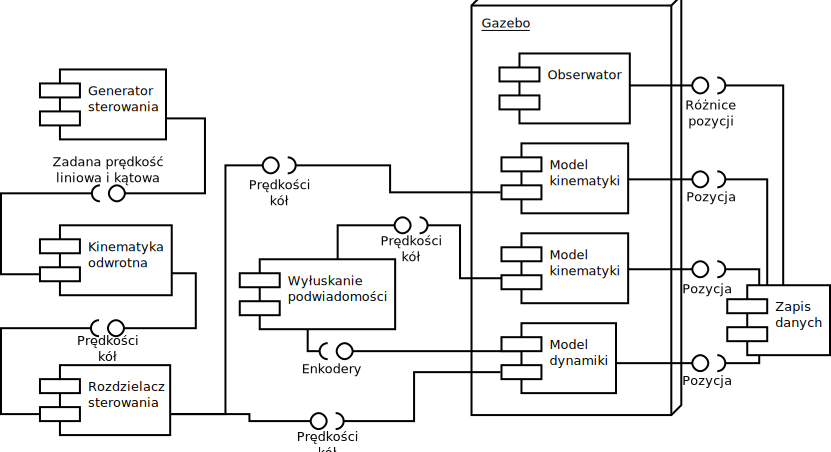
\includegraphics[width=\textwidth]{uml/comparison.pdf}
			\caption{Połączenie pakietów w teście porównującym modele.}
		\label{uml:comparison}
	\end{figure}
	
	\subsection{Porównanie modeli}
		Za pomocą pakietu do nadawania sterowania, opisanego w sekcji \ref{sec:gramofon}, nadano trasę o kształcie przedstawionym na rysunku \ref{plot:comparison_xy}.
		W tym teście robot kolejno poruszał się:
		\begin{enumerate}
			\item W przód z prędkością 0,25 \si{\metre\per\second} przez 5 \si{\second}.
			\item W prawo z prędkością $\pi/32$ \si{\metre\per\second} oraz prędkością kątową o $\pi/32$ \si{\radian\per\second} wokół osi Z, przez 8 \si{\second}.
			\item W tył z tą samą prędkością i przez ten sam czas, jak w punkcie 1.
			\item W prawo z prędkością $\pi/16$ \si{\metre\per\second} oraz prędkością kątową $\pi/32$ \si{\radian\per\second} wokół osi Z, przez 8 \si{\second}.
		\end{enumerate}
		Powyższe akcje wykonał czterokrotnie.
		
		\begin{figure}[H]
			\centering
			\includegraphics[width=\textwidth]{plots/comparison_xy.pdf}
				\caption{Trasa modelu platformy w teście porównującym modele. Różnica między zadaną trasą, a trasą wyznaczoną przez enkodery, jest niewielka.}
			\label{plot:comparison_xy}
		\end{figure}
		
		\begin{figure}[H]
			\centering
			\includegraphics[width=\textwidth]{plots/comparison_xt.pdf}
				\caption{Składowa pozycji modelu wzdłuż osi X w czasie.}
			\label{plot:comparison_xt}
		\end{figure}
		
		\begin{figure}[H]
			\centering
			\includegraphics[width=\textwidth]{plots/comparison_yt.pdf}
				\caption{Składowa pozycji modelu wzdłuż osi Y w czasie.}
			\label{plot:comparison_yt}
		\end{figure}
		
		\subsubsection{Dokładność odometrii}
			\label{sec:test_odometry}
			Trasa obliczana na podstawie prędkości kątowej kół, byłaby identyczna do zadanej trasy w przypadku gdyby koła obracałyby się dokładnie z zadanymi prędkościami kątowymi.
			To wymagałoby, aby silniki kół posiadały nieskończony moment siły, lub na tyle duży, aby opór obrotu, spowodowany tarciem, nie wpływał 
			znacząco na ich prędkość kątową. Innymi słowy, nawet jeśli platforma uderzyłaby w przeszkodę, koła nadal powinny obracać się zgodnie z zadanymi wartościami.
			To nie oznacza, że rzeczywista trasa robota jest zgodna z obliczoną z odometrii, gdyż uwzględnia także poślizgi kół, czego enkodery nie są w stanie wykryć.
			
			Różnice w pozycji zadanej, a pozycji obliczonej za pomocą danych wygenerowanych przez enkodery biorą się z tego, że
			silniki mogą nie mieć wystarczającej mocy, aby nadać kołom odpowiednie prędkości i przeciwdziałać oporom.
			Ponieważ założono dużą moc silników, jak zostało to opisane w sekcji \ref{sec:motors}, modelowane koła są mniej podatne na opory, a co za tym idzie, 
			ich prędkość będzie bardziej zbliżona do prędkości zadanej i także trasa wyznaczona w ten sposób z odometrii będzie niemalże pokrywać się z zadaną trasą.
			
			Zauważalne różnice pomiędzy przebiegami trasy odometrycznej i zadanej pojawiają się przy wywoływaniu dużych przyspieszeń i poślizgów na modelu platformy.
			
		\subsubsection{Trasa modelu dynamiki}
			Różnica pomiędzy położeniem modelu dynamiki, a kinematyki (położenia zgodnego z zadaną trasą), rośnie w czasie.
			Jest tak na skutek błędów numerycznych maszyny do symulacji fizyki, braku systemu operacyjnego czasu rzeczywistego, braku zamodelowania wszystkich oporów i skomplikowanej budowy modelu.
			Model dynamiki uwzględnia współczynniki tarcia kół o podłoże i jest w stanie modelować ich poślizgi.
			
			\begin{figure}[h]
				\centering
				\includegraphics[width=\textwidth]{plots/comparison_dt.pdf}
					\caption{Różnica pomiędzy położeniem modelu dynamiki i modelem kinematyki modelującym zadaną pozycję i pozycję odometryczną.}
				\label{plot:comparison_dt}
			\end{figure}
			
			\begin{figure}[h]
				\centering
				\includegraphics[width=\textwidth]{plots/comparison_at.pdf}
					\caption{Różnica pomiędzy orientacją modelu dynamiki i modelem kinematyki modelującym zadaną pozycję i pozycję odometryczną.}
				\label{plot:comparison_at}
			\end{figure}
			
		\subsubsection{Zachowanie się modelu dynamiki}
			Na wykresie \ref{plot:comparison_dt} zamieszczono różnice między położeniami odpowiednich modeli.
			Różnice nie zmieniają się monotonicznie ze względu na zmiany kierunków prędkości liniowej robota i jego prędkości kątowej wokół osi Z.
			Dlatego też, zdarzają się przypadki w których model dynamiki zbliża się do modelu kinematyki (zadanej pozycji) po tym gdy oddalił się od niej już wcześniej.
			
			Różnica pomiędzy wykresami jest mała, gdyż na obie wartości wpływają poślizgi kół w trakcie pokonywania trasy.
			Enkodery są wstanie wykryć zwiększoną siłę tarcia kół o podłoże na skutek obliczenia różnicy zadanego obrotu, a faktycznego.
			Taka zwiększona siła tarcia towarzyszy nagłym zmianom prędkości platformy, tak samo jak poślizg, lecz to nie powoduje że na
			podstawie pomiarów z enkoderów da się bezpośrednio wyznaczyć wartości poślizgu.
			Inaczej mówiąc, przyspieszenia platformy powodują poślizgi i trudności w obrocie kołami na skutek sił tarcia, lecz korzystając z danych z enkoderów można wyznaczyć
			jedynie opory obrotu kół.
			
			Przykładowe różnice pomiędzy wykresami występują na przykład w 15 sekundzie ruchu. 
			W tym miejscu nastąpił nagły zwrot bazy, który spowodował tarcie, a co za tym idzie i zwiększony opór ruchu obrotowego kół.
			Ten opór został wykryty przez enkodery, lecz poślizg nadal wpłynął na pozycję modelu dynamiki w większym stopniu.
			Dlatego też różnica między pozycją odometryczną, a pozycją modelu dynamiki wzrosła mniej, niż różnica pomiędzy pozycją modelu dynamiki, a pozycją wynikającą z zadanej trasy.
			
			Na wykresie \ref{plot:comparison_at} są pokazane różnice pomiędzy kątem obrotu wokół osi Z tych modeli.
			Podobnie, jak w przypadku położenia, bazując na danych z enkoderów, można obliczyć zmiany kierunku ruchu platformy.
			Na zmianę różnicy kąta obrotu nie wpływają jedynie zmiany prędkości kątowej, a również losowy kąt obrotu nadany platformie w przypadku poślizgów.
			Można zauważyć, że różnica między orientacją modelu dynamiki, a orientacją wyliczoną na podstawie odometrii zwykle zmienia się mniej dynamicznie od 
			różnicy między modelem dynamiki, a zadaną pozycją.
			
	\subsection{Powtarzalność testów}
		Zadano modelowi jazdę z różnymi prędkościami po trasie kwadratu, wyznaczona trasa została przedstawiona na rysunku \ref{plot:repetitions_xy}.
		
		\begin{figure}[H]
			\centering
			\includegraphics[width=\textwidth]{plots/repetitions_xy.pdf}
				\caption{Trasa modeli platformy, poruszających się z różną prędkością liniową po trasie kwadratu. W tym eksperymencie nie nadano prędkości kątowej.}
			\label{plot:repetitions_xy}
		\end{figure}
		
		Eksperyment pokazuje, że zależnie od prędkości przejazdu, mogą występować niedokładności ruchu. Dzieje się to głównie w kierunku Y, gdyż ruch
		platformy w kierunku X jest zawsze podobny. Im wolniej platforma się porusza, tym mniejszą odległość pokonuje w odpowiednio dłuższym czasie. 
		Tak jest na skutek wewnętrznego działania maszyny do symulacji fizyki. Potrzeba dokładniejszych testów, aby stwierdzić bezpośredni powód takiego zachowania.
		
		Kilkukrotne wykonanie tego samego eksperymentu pokazuje, że różnica tras pomiędzy przejazdami nie jest aż tak duża.
		 
\section{Porównanie modelu z robotem}
	\subsection{Trasa bez rotacji}
		\label{sec:test_velmobil}
		Za pomocą generatora sterowania, zadano platformie ruch po trasie kwadratu w prędkością 0,1 \si{\metre\per\second}, zaczynając od ruchu wzdłuż osi X.
		Zapisano dane generowane przez enkodery, obliczaną odometrię, pomiary skanerów laserowych oraz samo sterowanie.
		Następnie, używając tych samych danych, przeprowadzono identyczny eksperyment na modelu, łącząc pakiety w sposób pokazany na rysunku \ref{uml:comparison}.
		Korzystając z pakietu \texttt{laser\_scan\_matcher}, obliczono rzeczywistą pozycję platformy, korzystając z danych skanerów laserowych.
		Określenie pozycji jest obarczone błędem, wynikającym
		z błędów pomiarowych czujników, stąd obliczona trasa nie składa się z odcinków i posiada szum.
		Trasy modeli i platformy pokazano na wykresie \ref{plot:velmobil_xy}.
		
		\begin{figure}[H]
			\centering
			\includegraphics[width=\textwidth]{plots/velmobil_xy.pdf}
				\caption{Trasa modeli robota przy jeździe po trasie kwadratu.}
			\label{plot:velmobil_xy}
		\end{figure}
		
		\begin{figure}[H]
			\centering
			\includegraphics[width=\textwidth]{plots/velmobil_xt.pdf}
				\caption{Składowa pozycji modeli wzdłuż osi X.}
			\label{plot:velmobil_xt}
		\end{figure}
		
		\begin{figure}[H]
			\centering
			\includegraphics[width=\textwidth]{plots/velmobil_yt.pdf}
				\caption{Składowa pozycji modeli wzdłuż osi Y.}
			\label{plot:velmobil_yt}
		\end{figure}
		
		\begin{figure}[H]
			\centering
			\includegraphics[width=\textwidth]{plots/velmobil_xy_s.pdf}
				\caption{Przybliżenie wykresu \ref{plot:velmobil_xy}}
			\label{plot:velmobil_xy_s}
		\end{figure}
		
		Charakterystyczną cechą wykresu jest to, że robot przejechał mniejszą odległość wzdłuż osi X, niż wzdłuż osi Y.
		Może być to spowodowane różnicą w wyjściowym współczynniku tarcia kół w zależności od wyjściowego wektora prędkości kół.
		Zgodnie z cechą kół, opisaną w sekcji \ref{sec:robot_movement}, rolki kół obracają się z największą prędkością przy ruchu w bok, a co za tym idzie, w ruchu ma udział także
		ich tarcie obrotowe. Przy ruchu w przód, rolki nie obracają się, więc i to dodatkowe tarcie nie wpływa na ruch platformy.
		Dlatego też platforma pokonała mniejszą odległość w jednym z kierunków.
		
		Model dynamiki doznał poślizgu w trakcie 30 sekundy ruchu, która nadała mu niespodziewaną zmianę orientacji, przez co różnica w odległości od zadanej trasy znacząco wzrosła.
		
		\subsubsection{Nagła zmiana kierunku jazdy}
			Na wykresie \ref{plot:velmobil_xy_s} przedstawiono przybliżenie trasy modeli i robota w trakcie drugiego skrętu.
			Opisane niżej cechy są szczególnie dobrze widoczne na wektorowych wykresach w przypadku dokumentu elektronicznego.
			\begin{description}
				\item[Zadana trasa] nie pokrywa się dokładnie z przewidzianą trasą kwadratu, następują jej nieznaczne odchylenia.
				Jest to spowodowane działaniem symulacji i programu generującego sterowanie na systemie operacyjnym, który nie był systemem czasu rzeczywistego.
				Dodatkowo, pakiety sieciowe, zawierające wiadomości ROSa, przesyłane były przez sieć Ethernet, która nie gwarantuje przesyłu w deterministycznym czasie.
				To powoduje, że obliczona trasa nie koniecznie pokrywa się z zadaną trasą. Co więcej, na skutek niedeterministycznego przekazywania wiadomości przez strumienie komunikacyjne w czasie symulacji, każdy model i platforma mogły otrzymać nieco inne sterowanie, a co za tym idzie, różnice pomiędzy ich położeniami mogły być spowodowane tym efektem.
				\item[Odometria modelu] Jak wspomniano w sekcji \ref{sec:test_odometry}, trasa obliczona na jej podstawie niemal pokrywa się z zadaną trasą. 
				Jednakże, w trakcie nagłej zmiany kierunku ruchu, tarcie kół spowodowało nieznaczną różnicę prędkości kół w stosunku do zadanych wartości, co jest 
				wykryte jako ścięcie wykresu w kierunku Y. W przypadku modelu jest ono bardzo niewielkie, ale w tym samym kierunku, jak obliczone przez odometrię robota.
				To oznacza, że model enkoderów działa poprawnie, lecz być może jego parametry, czyli moment siły kół lub tarcie rolek nie są odpowiednio dobrane.
				\item[Model dynamiki] wykazał bezwładność w trakcie ruchu, to znaczy, jego prędkość liniowa w kierunku osi Y nie wzrosła natychmiastowo,
				lecz pod wpływem przyspieszenia, tak samo prędkość w kierunku X, która także nie spadła natychmiast.
				Jest to widoczne jako zaokrąglenie na wykresie.
				Opóźnienie w kierunku X było większe, niż przyspieszenie w kierunku Y, tzn. model szybciej wyhamował składową X prędkości liniowej, niż nadał zadaną składową Y prędkości liniowej, co się objawia jako wydłużenie trasy w danym kącie. Takie samo zachowanie wykazały trasy odometrii.
				\item[Skaner laserowy] Ponieważ pomiar z tego czujnika jest obarczony dużym błędem oraz małą częstotliwością pomiarów, nie można jednoznacznie określić bezpośredniego zachowania platformy w trakcie skrętu.
				\item[Odometria robota] Korzystając z enkoderów, program sterujący platformą obliczył jej pozycję. Nie jest to dokładna pozycja platformy, jaka jest określona przez skaner laserowy, lecz trasa wyznaczona tym sposobem jest zbliżona do zadanej trasy tak samo, jak trasa odometrii modelu. 
				Wykazuje takie same własności w trakcie skrętu, jak jej model, tylko w większym stopniu. Różnica w przyspieszeniu i opóźnieniu robota wskazuje, że 
				robot szybciej hamuje w kierunku X, niż przyspiesza w kierunku Y. Taki sam efekt występuje po drugiej stronie trasy, przy trzecim skręcie, lecz nie w drugim skręcie.
			\end{description}

	\subsection{Trasa z rotacją}
		\label{sec:test_velmobil_rot}
		Sterowanie robotem odbyło się w sposób podobny do testu \ref{sec:test_velmobil}, z tą różnicą, że przy wcześniejszej zmianie kierunku prędkości liniowej obracano platformą o 90° wokół osi Z. To znaczy, że platforma poruszała się w prawo z prędkością 0,1 \si{\metre\per\second}, a następnie obróciła o 90° 
		z prędkością kątową $\pi/20$ \si{\radian\per\second} i ponownie poruszała się w kierunku -X lokalnego układu współrzędnych.
		Trasa takiego przejazdu została przedstawiona na wykresie \ref{plot:velmobil_rot_xy}.
		Można na niej zauważyć poślizg przy ruszaniu platformy, który nadał jej losowy kąt obrotu.
		
		\begin{figure}[H]
			\centering
			\includegraphics[width=\textwidth]{plots/velmobil_rot_xy.pdf}
				\caption{Trasa modeli robota przy jeździe po trasie kwadratu z nadaniem prędkości kątowej wokół osi Z.}
			\label{plot:velmobil_rot_xy}
		\end{figure}
		
		\begin{figure}[H]
			\centering
			\includegraphics[width=\textwidth]{plots/velmobil_rot_xt.pdf}
				\caption{Składowa pozycji modeli wzdłuż osi X.}
			\label{plot:velmobil_rot_xt}
		\end{figure}
		
		\begin{figure}[H]
			\centering
			\includegraphics[width=\textwidth]{plots/velmobil_rot_yt.pdf}
				\caption{Składowa pozycji modeli wzdłuż osi Y.}
			\label{plot:velmobil_rot_yt}
		\end{figure}
		
		\begin{figure}[H]
			\centering
			\includegraphics[width=\textwidth]{plots/velmobil_rot_xy_s.pdf}
				\caption{Przybliżenie wykresu \ref{plot:velmobil_rot_xy}}
			\label{plot:velmobil_rot_xy_s}
		\end{figure}
	
		W tym przypadku nie ma informacji o odometrii wygenerowanej przez robota, gdyż nie obsługuje ona poprawnie rotacji platformy.
		
		Na przybliżeniu wykresu (rysunek \ref{plot:velmobil_rot_xy_s}) widać moment jak model dojechał do odpowiedniej pozycji i zaczął się obracać wokół osi Z. 
		Wykres pokazuje, że obrót następował wokół punktu znajdującego się o około 0,5 \si{\centi\metre} na prawo od środka modelu platformy.
		Nie jest wiadome, dlaczego tak się stało, gdyż model jest zdefiniowany symetrycznie, a środek układu współrzędnych, względem którego rysowany jest wykres, znajduje się 
		na środku platformy.
		Według enkoderów, punkt obrotu znajdował się z kolei na lewo od środka platformy.
		Takie zachowanie może być spowodowane na przykład asymetrią siatki definiującej kształt platformy, kolejnością obliczeń wykonywanych przy symulowaniu ogniw 
		obiektu lub innymi własnościami maszyny do symulacji fizyki.
	
\section{Jednostka inercyjna}
	\label{sec:test_imu}
	W trakcie powyższych testów zabrano również dane wygenerowane przez jednostkę inercyjną oraz jej model.
	\subsection{Akcelerometr}
		Ten czujnik zmierzył przyspieszenia modelu w trakcie testu \ref{sec:test_velmobil}.
		
		\begin{figure}[H]
			\centering
			\includegraphics[width=\textwidth]{plots/imu_xy.pdf}
				\caption{Porównanie odczytów pomiaru przyspieszenia liniowego jednostki inercyjnej, jej modelu i filtra redukującego szum.}
			\label{plot:imu_xy}
		\end{figure}
		
		W trakcie testu następowały kolejne przyspieszenia i opóźnienia bazy w zadanych kierunkach, to widać jako impulsy na wykresie \ref{plot:imu_xy}.
		Na początku platforma zaczęła poruszać się w kierunku -X i w tą stronę zostało nadane pierwsze przyspieszenie.
		Nie jest znana jego dokładna wielkość, gdyż zadany kierunek prędkości zmienił się w ciągu jednej wiadomości.
		
		Drugi impuls został wygenerowany w trakcie pierwszego skrętu bazy.
		Zadziałało przyspieszenie zmieniające kierunek prędkości liniowej platformy o 90°, co oznacza że impuls jest obrócony o 45° względem układu współrzędnych.
		Impuls wystąpił w kierunku (X,-Y). 
		Jest to wypadkowa przyspieszenia bazy w kierunku -Y i opóźnienia w kierunku poprzedniego kierunku jazdy, czyli -X.
		
		Podobna zmiana prędkości nastąpiła jeszcze dwa razy, generując kolejne, symetryczne impulsy.
		
		Na koniec platforma zatrzymała się, generując opóźnienie w kierunku Y, co także widać na wykresie w postaci przyspieszenia w przeciwnym kierunku.
		
		Porównując dane wygenerowane przez jednostkę inercyjną nie widać zależności, jednak zastosowanie prostego uśrednienia pakietem opisanym w sekcji \ref{sec:odszumiacz} powoduje, że impulsy wygenerowane przez robota również są widoczne. Każda uśredniona wartość jest średnią z 40 poprzednich.
		
		Po przefiltrowaniu danych z robota, można zaobserwować jak każdy impuls ma kształt półksiężyca, na początku każdej zmiany prędkości opóźnienie ma kierunek równoległy do wektora prędkości, zatrzymując robota, następnie wolniejsze przyspieszenie nadaje nowy kierunek, a potem następuje reakcja korpusu i gasnące drgania w nowym kierunku. 
		Zamodelowanie tej własności mogłoby okazać się bardzo trudne, prawdopodobnie należałoby nadać dodatkowe ogniwa do robota i połączyć je więzami sprężynowymi.
		
		Szum, jakimi są obarczone zamodelowane dane spowodowany jest potrzebą różniczkowania prędkości liniowej modelu, obliczanej dyskretnie przez maszynę do symulacji fizyki. 
		Wartości mas i momentów bezwładności ogniw modelu mocno wpływają na kształt impulsów, kolerację
		osi i szum na wykresie. 
		Nie jest technologicznie możliwe zamodelowanie jednostki inercyjnej pozbawionej szumu ze względu na błędy numeryczne, algorytmy użyte w maszynie
		symulującej fizykę i system operacyjny na którym pracuje symulator.
		
		\begin{figure}[H]
			\centering
			\includegraphics[width=\textwidth]{plots/imu_xy_n.pdf}
				\caption{Porównanie odczytów pomiaru przyspieszenia liniowego modeli jednostki inercyjnej z dodanym szumem i bez.}
			\label{plot:imu_xy_n}
		\end{figure}
		
		Na wykresie \ref{plot:imu_xy} widać szum generowany przez jednostkę inercji w trakcie ruchu jednostajnego. Jest on mniejszy od niedokładności generowanych
		przez model. Jednakże, w trakcie działania przyspieszenia, model jednostki inercyjnej wygenerował większy impuls, niż urządzenie.
		Do wykrycia kierunków impulsów nie potrzebna jest filtracja danych, ale taka filtracja okazała się niezbędna w przypadku danych zebranych z jednostki inercyjnej.
		
		Aby przybliżyć zachowanie się modelu jednostki inercyjnej w trakcie ruchu z prędkością jednostajną, do odczytów urządzenia, dodano dodatkowy szum o rozkładzie normalnym.
		Jego parametry określone są w tabeli \ref{tab:imu_noise}.
		Na rysunku \ref{plot:imu_xy_n} przedstawiono porównanie generowanych przez model danych z szumem i bez.
		Można zauważyć silną korelację modelu jednostki inercyjnej w zależności od kierunku prędkości liniowej robota. 
		Korelacja jest także silnie uzależniona od parametrów modelu dynamiki. Występują bazowe drgania w dwóch kierunkach.
		Niestety, amplituda bazowych drgań w modelowanym czujniku jest większa niż amplituda szumu rzeczywistej jednostki, w dodatku występuje korelacja wzdłuż dwóch prostych.
		Widać to na wykresach przebiegu czasowego \ref{plot:imu_yt} i \ref{plot:imu_xt}.
		
		\begin{figure}[H]
			\centering
			\includegraphics[width=\textwidth]{plots/imu_xt.pdf}
				\caption{Porównanie składowej X pomiarów przyspieszenia liniowego jednostki inercyjnej, jej modelu i filtra redukującego szum.}
			\label{plot:imu_xt}
		\end{figure}
		
		\begin{figure}[H]
			\centering
			\includegraphics[width=\textwidth]{plots/imu_yt.pdf}
				\caption{Porównanie składowej Y pomiarów przyspieszenia liniowego jednostki inercyjnej, jej modelu i filtra redukującego szum.}
			\label{plot:imu_yt}
		\end{figure}
		
		Aby użyć tego czujnika do obliczania pozycji, trzeba wpierw użyć bardziej zaawansowanego algorytmu odszumiającego i wyprowadzić eksperymentalnie zależności pomiędzy czujnikami
		osi (macierz kowariancji).
		
		Na wykresach \ref{plot:imu_xt} i \ref{plot:imu_yt} widać jak w około 15 sekundzie ruchu na platformę zadziałała nagła zmiana prędkości liniowej.
		Wykres przebiegu trasy nie wskazuje, jakoby zdarzyła się tam nagła zmiana prędkości.
	
	\subsection{Żyroskop}
		Czujnik prędkości kątowej korzysta z żyroskopu i zwraca prędkość kątową we wszystkich trzech osiach.
		Ponieważ jednak platforma porusza się po płaskim terenie, wymagany jest jedynie czujnik mierzący obrót wokół osi Z, czyli w górę.
		Drugą osią wykresu może być zatem czas nadania pakietu. Te dane zostały zebrane w trakcie testu \ref{sec:test_velmobil_rot}.
		
		\begin{figure}[H]
			\centering
			\includegraphics[width=\textwidth]{plots/angimu_at.pdf}
				\caption{Porównanie prędkości kątowej wokół osi Z, wygenerowanej przez jednostkę inercyjną i jej model.}
			\label{plot:angimu_at}
		\end{figure}
		
		\begin{figure}[h]
			\centering
			\includegraphics[width=\textwidth]{plots/angimu_at_w.pdf}
				\caption{Porównanie danych wygenerowanych przez model jednostki inercyjnej i prędkości kątowej wokół osi Z modelu.}
			\label{plot:angimu_at_w}
		\end{figure}
		
		Ponieważ maszyna do symulacji fizyki wewnętrznie posiada informację o prędkościach obiektów, model tego czujnika po prostu zwraca gotowe dane. 
		To powoduje, że praktycznie pozbawiony jest szumu, co można zauważyć na wykresie \ref{plot:angimu_at_w}.
		Aby zatem polepszyć jakość symulacji, dodano sztuczny szum do generowanych danych, zgodnie z tabelą \ref{tab:imu_noise}.
		W ten sposób wykresy są do siebie bardziej zbliżone.
		
		Jednak niektórych własności czujnika nie da się zamodelować tak łatwo. Po pierwsze, szum czujnika nie do końca ma rozkład normalny.
		Z wykresu można zobaczyć, że dane prawdopodobnie korelują z częstotliwościami obrotu kół.
		Dodatkowo, nagła zmiana prędkości kątowej powoduje zauważalny skok na wykresie, co w symulowanych danych jest znacznie mniej widoczne.
		Może być to spowodowane drganiem robota przy nagłych zmianach prędkości kątowej, co nie jest uwzględnione w modelu.
		
		
		
	
	

%TODO różnica współczynników tracia w bok i do przodu

\chapter{Podsumowanie}
\label{sec:ending}

Wszystko ładnie pięknie.
%TODO coś napisać

\begin{thebibliography}{0}

% stosowanie_modelu.pdf
\bibitem{kinematic_modeling}
P. Muir, C. Neuman ``Kinematic modeling for feedback control of an omnidirectional wheeled mobile robot'', 
Proceedings, IEEE International Conference in Robotics and Automation, 
Vol 4. pp. 1772-1778, 1987.

% koła.pdf
\bibitem{wheels}
Mihai Olimpiu Tătar, Cătălin Popovici, Dan Mândru, Ioan Ardelean, Alin Pleşa ``Design and development of an autonomous omni-directional mobile robot with Mecanum wheels'',
Conference: 2014 IEEE International Conference on Automation, Quality and Testing, Robotics (AQTR)

% paletobot.pdf
\bibitem{paletobot}
Matthieu LAMY ``Mechanical development of an automated guided vehicle'',
Master of Science Thesis MMK 2016:153 MKN 171,
KTH Industrial Engineering and Management,
Machine Design,
SE-100 44 Sztokholm

% matematyka_rolki.pdf
\bibitem{rollers}
Anton Gfrerrer ``Geometry and kinematics of the Mecanum wheel'',
Graz University of Technology, Institute of Geometry, Kopernikusgasse 24, 8010 Graz, Austria,
Computer Aided Geometric Design 25(9):784-791

% silny_robot.pdf
\bibitem{heavy}
Li Xie, Christian Scheifele, Weiliang Xu, Karl A. Stol ``Heavy-Duty Omni-Directional Mecanum-Wheeled Robot for Autonomous Navigation'',
DOI: 10.1109/ICMECH.2015.7083984

% hamowanie.pdf
\bibitem{braking}
Viktor Kálmán ``On modeling and control of omnidirectional wheels'',
PhD. dissertation, Budapest University of Technology and Economics,
Department of Control Engineering and Information Technology

% ruchome_osie.pdf
\bibitem{extra_axis}
Jae-Bok Song, Kyung-Seok Byun
``Design and Control of a Four-Wheeled Omnidirectional Mobile Robot with Steerable Omnidirectional Wheels'',
Journal of Robotic Systems 21(4):193-208, Kwiecień 2004

\bibitem{gazebo_website}
Strona internetowa symulatora Gazebo. \\
\url{http://gazebosim.org}

\bibitem{vrep_website}
Strona internetowa symulatora V-Rep. \\
\url{http://coppeliarobotics.com}

\bibitem{ros_website}
Strona internetowa platformy programistycznej \emph{Robot Operating System}. \\
\url{http://www.ros.org}

\bibitem{sdf_website}
Strona internetowa standardu SDF. \\
\url{http://sdformat.org/spec}

\bibitem{ode_contact}
Dokumentacja maszyny ODE z wyjaśnieniem działania kolizji. \\
\url{http://ode-wiki.org/wiki/index.php?title=Manual:_Joint_Types_and_Functions#Contact}

\end{thebibliography}

\end{document} 
